%% LyX 2.4.2.1 created this file.  For more info, see https://www.lyx.org/.
%% Do not edit unless you really know what you are doing.
\documentclass{article}
\usepackage[T1]{fontenc}
\usepackage[utf8]{inputenc}
\usepackage{color}
\usepackage{float}
\usepackage{amsmath}
\usepackage{graphicx}
\usepackage{geometry}
\geometry{verbose,tmargin=1in,bmargin=1in,lmargin=1in,rmargin=1in}
\usepackage{esint}

\makeatletter
%%%%%%%%%%%%%%%%%%%%%%%%%%%%%% User specified LaTeX commands.
%\usepackage{epstopdf} % to include .eps graphics files with pdfLaTeX
\usepackage{flafter}   % Don't place floats before their definition
%\usepackage{topcapt}  % Define \topcation for placing captions above tables (not in gwTeX)

\usepackage{xurl}      % better URL setting, uses old url package

\usepackage{xcolor}
\definecolor{darkblue}{rgb}{0,0,0.4}
\usepackage[]{hyperref} % Generates all cross references
\hypersetup{            % Setting options for hyperref package
	breaklinks=true,    % break line with long hyperlinks
	colorlinks=true,    % coloured links
	linkcolor=blue,
	filecolor=magenta,
	urlcolor=darkblue,
	citecolor=blue,
	backref=page
} 

\usepackage{memhfixc}  % remove conflict between the memoir class & hyperref
\usepackage{pdfsync}   % enable tex source and pdf output syncronicity

\usepackage{memhfixc}  % remove conflict between the memoir class & hyperref
\usepackage{pdfsync}   % enable tex source and pdf output syncronicity

\usepackage{alltt}

% \usepackage{listings}
% \usepackage{xcolor}

% \lstdefinestyle{mystyle}{
%   language=Python,
%   numbers=left
% }

% Put lstset here, after lstdefinestyle
% \lstset{style=mystyle}

\makeatother

\usepackage[dutch]{babel}
\usepackage{listings}
\lstset{language=Python,
extendedchars=false,
frameround=fttt,
numbers=left,
% line numbers use none,
numberstyle={\tiny},
stepnumber=2,
% line numbers only every so many,
numbersep=9pt,
% how far line numbers from text?,
showspaces=false,
showstringspaces=false,
showtabs=false,
tab={\rightarrowfill},
basicstyle={\small},
keywordstyle={\color{blue}},
commentstyle={\color{green}},
stringstyle={\ttfamily \color{magenta}},
identifierstyle={\color{black}}}
\begin{document}

\title{Verlaging in een gebied met vrije afwatering}
\author{T.N.Olsthoorn}
\date{06-04-2025}
\maketitle
\begin{center}
\includegraphics[width=0.6\textwidth]{/Users/Theo/Entiteiten/Hygea/2022-AGT/jupyter/images/example_fdm3_1D+FDR}
\par\end{center}

\newpage{}

\tableofcontents{}

\newpage{}

\section{Samenvatting en conclusies}

Er zijn veel gebieden met vrije drainage, meestal lagere waarin het
oppervlaktewater grondwater afvoert afkomstig van aangrenzende hoger
gelegen gebieden met diepere grondwaterstanden waarin geen oppervlaktewater
aanwezig is. beekdalen zijn hiervan een voorbeeld, maar ook oorspronkelijke
moerassen, waar het neerslagwater niet diep kan infiltreren maar min
of meer direct via het oppervlaktewaterstelsel wordt afgevoerd. Waar
geen water extern kan worden aangevoerd, is de afvoer van het oppervlaktewater
volledig afhankelijk van de aanvoer van grondwater. Deze afvoer ademt
mee met fluctuerende grondwaterstanden die kenmerkend zijn voor de
verschillende seizoenen en is bovendien gevoelig voor verlaging van
diezelfde grondwaterstanden door onttrekkingen voor uiteenlopende
doelen als drinkwatervoorziening, bemaling of irrigatie. Zulke gebieden
met vrije drainage zijn kwetsbaar voor menselijk ingrijpen en dat
geldt uiteraard ook voor de daarin aanwezige natuur.

Het berekenen of modelleren van de verlaging van de grondwaterstanden
en de afvoer in zulke gebieden is minder recht-toe-recht-aan omdat
met de daling van de grondwaterstand niet alleen de afvoer zelf afneemt,
maar ook het waterpeil in de open waterlopen. Het slootpeil stijgt
en daalt daar met de grondwaterstand en daarmee met de lek naar de
sloten, terwijl infiltratie vanuit de sloten in vrij afwaterende gebieden
niet mogelijk is. De gebruikelijke modellering gaat uit van een vaste
drainagebasis. Omdat de drainagebasis, dat wil zeggen het slootpeil,
in vrij afwaterende gebieden meezakt met de verlaging van de grondwaterstand
is de verlaging van de grondwaterstand zelf ook groter dan bij vaste
drainagebasis het geval zou zijn. Het zal dus voor een adequate modellering
van belang zijn hier rekening mee te houden. Hoewel voor situaties
met vaste drainagebasis analytische oplossingen (berekeningen) mogelijk
zijn, is dat voor situaties met variabele drainagebasis niet het geval.
We kunnen deze alleen modelleren met een grondwatermodel waarin het
gedrag van het slootpeil is verdisconteerd.

Meenemen van het gedrag van het oppervlaktewater is slechts beperkt
mogelijk zonder het grondwatermodel te koppelen aan een oppervlaktewatermodel
dat behalve met de lokale afvoer naar de sloten ook rekening houdt
met wat bovenstrooms gebeurt, zodat water dat bovenstrooms naar het
oppervlaktewater lekt eventueel benedenstrooms kan infiltreren. Een
dergelijke aanpak gaat hier veel te ver. Daarom wordt in dit document
het slootpeil afhankelijk gemaakt van de lek ter plekke zonder te
kijken naar het gehele bovenstroomse gebied. Dit is een benadering
die in de praktijk veelal voldoende zal zijn.

Drainage leidt tot een grondwaterstand-afvoerrelatie. Bij een vast
drainpeil en vaste drainageweerstand is dat een verticale lijn zolang
het grondwater zich beneden het drainagepeil bevindt (dat wil zeggen
geen afvoer) en een rechte schuine lijn wanneer de grondwaterstand
zich ter plaatse boven het drainagepeil bevindt (dat wil zeggen vaste
drainageweerstand). In de praktijk kan de drainageweerstand afnemen
met toenemende grondwaterstand, waar door de grondwaterstand-afvoerrelatie
een kromme lijn wordt. Dit is ook het geval bij vrije drainage. De
afvoer neemt dan lineair toe met de grondwaterstand, zodra de grondwaterstand
zich boven de slootbodem bevindt. Het slootpeil speelt dan geen rol
meer in de modellering, die is als het ware uit de vergelijking geëliminieerd.
Vrije drainage kan zodoende met een standaard model zoals Modflow
worden gesimuleerd door de drainageweerstand te laten afnemen met
de grondwaterstand, via een op deze wijzen vastgelegde grondwaterstand-afvoerrelatie
(\cite{MF6}).

Dit document leidt de vrije drainage uit vanaf de basis, wat leidt
tot modelrandvoorwaarden voor de vrije drainage die direct in een
model kunnen worden geïmplementeerd en arbitraire keuzen voor de grondwaterstandafvoerrelatie
zoveel mogelijk elimineren. Bovendien wordt uitgegaan van gegevens
die gemakkelijk in het veld kunnen worden vastgesteld. Deze gegevens
zijn grondwaterstand, slootpeil, slootdiepte, en neerslagoverschot
in de referentiesituatie, dus meestal de gemiddelde situatie en wanneer
de drainageweerstand wordt berekend uit slootprofiel en slootbreedte
ook de slootbreedte en de gemiddelde slootafstand. Dit impliceert
dat de afgeleide en geïmplementeerde vrije drainage in twee variante
komt: A) waar de dainageweerstand wiskundig is opgelegd en B) waar
deze wordt berekend uit slootprofiel en slootdiepte. Uiteindelijk
zal het verschil tussen beide varianten niet groot blijken te zijn,
maar het verschil met de situatie met vaste drainagebasis is dat wel.

De vrije drainage is geïmplementeerd in een eindig differentie model,
als een type randvoorwaarde met de naam FDR (free drainage) naast
de bekende typen GHB (general head boundaries), DRN (drain boundaries)
en RIV (river boundaries). Hiermee zijn de resultaten met verschillende
randvoorwaarden gemakkelijk onderling te vergelijken in de voorbeelden
in dit document. De afgeleide en geïmplementeerde randvoorwaarde voor
vrije drainage kunnen direct in Modflow worden geïmplementeerd als
een afzonderlijk package. De relatie tussen grondwaterstand en afvoer
die de vrije drainage kenmerkt kan in Modflow ook worden opgelegd
door deze op te leggen als een gebroken lijn in de DRN module van
Modflow zelf. De afleiding in dit document helpt dan bij de keuze
van deze lijn.

In het algemeen is het belangrijk om vrije drainage mee te nemen in
de modellering van gebieden met oppervlaktewater dat meeademt met
de grondwaterstand, waarin grondwater alleen kan worden afgevoerd
maar niet aangevoerd. Dit kan alleen goed worden gemodelleerd met
een grondwatermodel aangezien er geen analytische oplossingen bestaan
die vrije drainage meenemen. Het grondwatermodel moet dit dan wel
kunnen. De in dit document uitwerkte aanpak doet dit transparant op
natuurlijke wijze en blijft zoveel weg van arbitraire keuzen. Door
bij de afleiding uit te gaan van gemakkelijk uit het veld verkrijgbare
gegevens, is implementatie in de praktijk transparant en eenvoudig.
Het is ten alle tijde mogelijk om de resultaten te vergelijken met
die van vaste drainage of de analytische oplossingen die daar wel
voor beschikbaar zijn.

\newpage{}

\part{Context en historie}

\section{Intro}

In een gebied met vrije afwatering, dus zonder de mogelijkheid van
kunstmatige toevoer van extern water of van peilbeheer, hangt het
slootpeil van de afvoer af, dat wil zeggen van de lek van het grondwater
naar de sloten. Zonder afvoer zijn de sloten droog en bij gemiddelde
afvoer is er een gemiddeld slootpeil. Hiervan kan een drainageweerstand
worden afgeleid, zijnde de gemiddelde stijghoogte van ht grondwater
boven het gemiddelde slootpeil gedeeld door de gemiddelde afvoer;
deze is in de regel gelijk aan het neerslagoverschot, en waar van
toepassing vermeerderd met de kwel.

Bij verlaging van de grondwaterstand, of dit nu komt door natuurlijke
processen of door grondwateronttrekking of peilwijziging, daalt de
afvoer en dus ook het slootpeil. Om het grondwater in een gebied met
vrije afwatering adequaat te kunnen modelleren zou een grondwatermodel
moeten worden gekoppeld aan een oppervlaktewatermodel. Een stap minder
complex is om het verband tussen afvoer en slootpeil als een vaste
relatie op te nemen in het grondwatermodel. Dat is wat in dit document
wordt uitgewerkt.

Bij afnemende afvoer daalt het slootpeil om uiteindelijk, bij afvoer
nul de slootbodem te bereiken. Hoe dat verband er precies uitziet
is niet bij voorbaat helemaal duidelijk, maar een verband zoals getekend
in figuur \ref{fig:afvoerrelaties} lijkt voor de hand te liggen.
De daling verloopt steeds sneller naarmate de slootdiepte verder afneemt.

De drainageweerstand is de ruimtelijk gemiddelde grondwaterstand minus
slootpeil ( = de drainagebasis) gedeeld door de gebiedsafvoer, zoals
het neerslagoverschot. Ook de drainageweerstand verandert met het
slootpeil en dus met de afvoer. De drainageweerstand definiëren we
voor het in de tijd gemiddelde neerslagoverschot, $N$, eventueel
plus kwel. Hij wordt oneindig groot wanneer het stijghoogte en daarmee
ook het slootpeil zijn gedaald tot op de slootbodem, en blijft dat
zolang de grondwaterstand daaronder zit.

Men kan deze variabele drainageweerstand als een vaste relatie opleggen,
zoals in het onderste plaatje van figuur \ref{fig:afvoerrelaties}
is weergegeven. Men kan de drainageweerstand echter ook berekenen
op basis van het slootprofiel en de actuele slootdiepte. Deze fysische
drainageweerstand bestaat uit een aantal bijdragen waarvan de radiale
weerstand, die ontstaat door contractie van stroomlijnen in de richting
van de sloot, mede wordt bepaald door de grootte van het natte contactvlak
tussen sloot en watervoerend pakket. Bij daling van de grondwaterstand
wordt dit contactvlak uiteindelijk nul, en de weerstand dus oneindig
groot. Zoals uit de uitgewerkte voorbeelden zal blijken zit er niet
heel veel licht tussen de uitkomsten berekend met een weerstand die
als vaste wiskundige relatie wordt opgelegd en een weerstand die wordt
berekend op basis van de grootte van genoemd contactvlak, dat afhangt
van de waterstand in de sloot.

\section{Aanpak van Blom / Ernst}

\cite{Blom73} and Ernst (\cite{Lou22}) behandelde vrije afwatering
in eerste instantie als een gebied met een bepaalde vaste drainageweerstand,
waarin hij de werking van het drainerende oppervlaktewater samenvatte.
Bij een onttrekking ontstaat een binnengebied waarbinnen de grondwaterstand
daalt tot beneden het niveau waarop de afwatering nul wordt, en een
buitengebied waar het ontwateringsstelsel nog wel een deel van het
neerslagoverschot afvoert. In het binnengebied voedt al het niet meer
afgevoerde neerslagoverschot het grondwater, en in het buitengebied
is dit een deel van het neerslagoverschot, dat bij een constante drainageweerstand
evenredig is aan de verlaging. De grens tussen beide gebieden ligt
waar de verlaging gelijk is aan $Nc$, het product van neerslagoverschot
$N$ en drainageweerstand $c$. De analytische formule die geldt voor
de stroming in het binnengebied is dan die van Verruijt, dat wil zeggen
Dupuit plus neerslagoverschot, en in het buitengebied die voor onttrekking
aan semi-gespannen grondwater volgens \cite{Glee30}.

De hierboven beschreven benadering kan geheel analytisch worden opgelost,
maar impliceert een lineair verband tussen verlaging en voeding en
een vast peil van het oppervlaktewater, het drainagepeil of de drainagebasis,
en een constante drainageweerstand zolang de grondwaterstand zich
boven het drainagepeil bevindt. In een vrij afwaterend gebied zijn
beide factoren echter niet constant. In de eerste plaats neemt de
drainagebasis, het slootpeil, toe met de afvoer. In de tweede plaats
verandert het slootprofiel met het slootpeil en is derhalve ook de
uittreeweerstand, en daarmee de drainageweerstand niet constant. In
het laatste deel van zijn rapport gaat \cite{Blom73} daarom uit van
een parabolisch verloop van de drainageweerstand en de drainagebasis
met de afvoer. Hij ijkt deze aan het grondwaterstandsafvoerverloop
voor enkele vrij afwaterende gebieden in de provincie Drenthe en toetst
dit aan een model waar deze parabolische, dus niet lineaire, benadering
was ingebouwd. Voor deze niet-lineare relaties waren en zijn geen
analytische oplossingen bekend, waardoor op een numeriek model moest
worden teruggevallen.

\section{Modflow}

In de afgelopen 50 jaar later hebben we veel ervaring opgedaan met
numerieke modellen van verschillende snit. Het meest gebruikte model,
dat ook veel opties heeft voor randvoorwaarden is Modflow. De nieuwste
versie, Modflow6, heeft intern een aanpak die het convergentiegedrag
sterk verbetert ten opzichte van voorgaande versies, waarin met name
het droogvallen en/of nat worden van oorspronkelijk droge rekencellen
frequent leidde tot het niet convergeren van de numerieke oplossing.
Dat is nu verleden tijd. Maar al vanaf de eerste versie van Modflow,
uit 1988, had het programma opties voor drains die alleen afvoeren
wanneer de grondwaterstand hoger is dan het niveau van de drains,
en voor rivieren waarin, zodra de stijghoogte daalt tot beneden de
rivierbodem, de infiltratie een maximum bereikt dat verder constant
blijft. Beide stijghoogterandvoorwaarden zijn niet-lineair omdat bij
infiltratie de voeding wordt beperkt of gelijk aan nul wordt. Tegenwoordig
kan de infiltratieweerstand bij drains in Modflow afhankelijk worden
gemaakt van de waterstand boven de drains. Daarmee kan een niet-lineaire
grondwaterstandafvoerrelatie worden gesimuleerd, die overeen komt
met een afvoerstelsel bestaande uit sloten uit verschillende categoriëen,
dus met verschillende breedtes en dieptes.

Met al deze opties is het wel mogelijk om de drainage- of lekweerstand
te afhankelijk te maken van de stijghoogte, maar nog steeds is het
drainageniveau daarbij constant, terwijl dat in de praktijk zeker
niet zo is. Hierna zal met name dit aspect van vrij afwaterende gebieden
worden meegenomen in de analyse.

Wanneer we de eerste aanpak van Blom vergelijken met wat we in Modflow
met de optie van drains kunnen doen, zal duidelijk worden dat beide
identiek zijn. In een vlak Modflowmodel dat is belegd met drains met
een weerstand die overeenkomt met de drainageweerstand en wordt belast
met een constant neerslagoverschot, voert elke drain-cel exact dit
neerslagoverschot af en wordt de stijghoogte uniform gelijk aan $\phi=h_{drain}+Nc$
. Voegen we een onttrekking toe, dan daalt de afvoer in evenredigheid
met de verlaging en de drainageweerstand, behalve voor rekencellen
waarin de verlaging groter is dan $Nc$. Daar valt de afvoer nu geheel
weg en is de netto voeding aan het pakket gelijk aan $N$ geworden.
Dit is exact de werking volgens het schema van \cite{Blom73} en is
derhalve al vanaf de eerste versie van Modflow in het programma aanwezig.

Het gebruik van de optie DRN in Modflow, is dus geschikt voor het
implementeren van afvoer van sloten zodra de grondwaterstand boven
het drainniveau uitkomt. Voor het regelen van de infiltratie van sloten
werkt dit niet. In de praktijk is de uittreeweerstand van sloten een
stuk kleiner dan de intreeweerstand. In Modflow kunnen we met de ,,general
head boundary'' optie (GHB) een uitwisseling tussen het model en
een slootpeil simuleren die evenredig is met het stijghoogteverschil
gedeeld door de weerstand. Bij de GHB optie wordt geen onderscheid
gemaakt tussen infiltratie vanuit en exfiltratie naar sloten. Door
de GHB optie te combineren met de DRN optie kan in Modflow uitwisseling
met sloten worden gesimuleerd, waarbij de uittreeweerstand lager is
dan de intreeweerstand. Dit wordt in de modelleringspraktijk vaak
toegepast. Voor vrij afwaterende gebieden waarin geen aanvoer van
buiten mogelijk is, en geen peil in de sloten kan worden gefixeerd,
is dit niet aan de orde. De RIV optie in Modflow werkt als de GHB
optie zolang de grondwaterstand hoger is dan de rivierbodem. Bij stijghoogten
beneden de rivierbodem blijft de infiltratie gelijk aan die bij het
bereiken van de rivierbodem. Dit weerspiegelt een onverzadigde zone
die daarbij onder de rivierbodem ontstaat. Zet men in de RIV optie
de waterstand in de rivier gelijk aan de hoogte van de rivierbodem,
dan werkt deze identiek aan de DRN optie. Door beide te combineren
kan men de drainage-weerstand op een gewenst niveau laten verspringen.
Volledige vrijheid ontstaat wanneer men meer DRN opties binnen een
enkele cel mag toepassen. Hetzelfde wordt bereikt door in Modflow
gebruik te maken van de optie om de relatie tussen afvoer en stijghoogte
als een gebroken lijn op te leggen. Deze veralgemeniseerde DRN-optie
is minder kunstmatig en geeft meer flexibiliteit. Maar geen van deze
opties biedt de mogelijkheid om ook het drainageniveau zelf te laten
oplopen met de afvoer/kwel.

\newpage{}

\part{Afleiding van de vrije drainage}

\section{Intro}

We zullen hierna op een natuurlijke wijze de relatie tussen stijghoogte,
slootpeil en afvoer afleiden en implementeren. We gaan hierbij uit
van gegevens die direct vanuit de veldsituatie op een gemakkelijke
manier kunnen worden verkregen. Dit betreft de stijghoogte, het slootpeil,
en het neerslagoverschot in de gemiddelde, zeg referentie-situatie,
en voorts de hoogte van de slootbodem. In de variant waarin we de
drainageweerstand berekenen op basis van het slootprofiel komen daar
de slootbreedte en de gemiddelde slootafstand nog bij. Dit zijn allemaal
gegevens die direct in het veld kunnen worden vastgesteld. Dit leidt
tot een nieuwe optie, FDR gedoopt, wat staat voor Free Drainage, die
aan Modflow kan worden toegevoegd, maar voorlopig nog alleen aanwezig
is in een eigen implementatie (Github).

\section{De lek vanuit het grondwater naar de sloten}

Kern van de vrije drainage is de lek of uittrede van het grondwater
naar de sloten in een gebied. Deze kan per eenheid van gebiedsoppervlak
worden beschreven met

\[
q=\frac{\phi-h}{c}
\]

Hierin is $q$ de afvoer per oppervlakteëenheid, $\phi$ de grondwaterstijghoogte,
$h$ het slootpeil (= de drainagebasis) en $c$ de uittrede-, drainage-
of lekweerstand, die hier als identiek worden beschouwd. Het slootpeil
en de lekweerstand hangen in vrij afwaterende gebieden van de afvoer
$q$ {[}m/d{]} naar de sloten af, zodat

\[
q=\frac{\phi-h\left(q\right)}{c\left(q\right)}
\]

Door de relaties $h\left(q\right)$ en $c\left(q\right)$ in een grondwatermodel
te gebruiken, kan het grondwatermodel rekening houden met natuurlijke
afwatering. Voorwaarde is wel dat het grondwatermodel met deze niet-lineaire
relaties convergeert.

We zullen verderop zien dat het variabele slootpeil $h$ kan worden
geëlimineerd ten gunste van het vaste niveau van de slootbodem $h_{0}$.

Figuur \ref{fig:afvoerrelaties} geeft in het bovenste plaatje de
situatie weer. Bij toenemende stijghoogte nemen het slootpeil en de
afvoer volgens een bepaald verband toe. We kiezen de gemiddelde afvoer
$q=N$ als referentie omdat we deze situatie direct in het veld kunnen
waarnemen.

\begin{figure}[h]
\centering
\includegraphics[width=0.8\textwidth]{../jupyter/images/vrije_afwatering}

\caption{\label{fig:afvoerrelaties}Relatie stijghoogte, slootpeil, drainageweerstand
en afvoer.}

\end{figure}


\section{Relatie tussen slootpeil en afvoer}

De vraag is hoe de relatie tussen slootpeil en afvoer eruit zou moeten
zien. Met afvoer zou taalkundig de afvoer in de langsrichting van
de sloot kunnen worden bedoeld, die uiteraard sterk afhankelijk is
van de afvoer uit bovenstrooms gebied. Daar kan echter alleen rekening
mee worden gehouden door het grondwatermodel direct te koppelen aan
een model voor het oppervlaktewater. Dat voert hier veel te ver. 

In dit document wordt met afvoer de kwel of lek of drainage bedoeld
vanuit het watervoerend pakket naar het oppervlaktewater, die in een
vrij afwaterend gebied optreedt zodra de grondwaterstand boven de
slootbodem uitstijgt. We zullen de afvoer vlakdekkend interpreteren,
zodat we geen individuele sloten hoeven mee te nemen in de analyse.
Zo'n beperking is voor het eindige differentie model niet van toepassing.

We mogen ervan uitgaan dat het gemiddelde slootpeil van een te modelleren
gebied bekend is. Het slootpeil mag ook zonder bezwaar ruimtelijk
variëren. We gaan er voorts van uit dat we dit slootpeil kunnen relateren
aan de gemiddelde afvoer, en dat die gemiddelde afvoer gelijk is aan
het neerslagoverschot $N$~{[}L/T{]}, eventueel vermeerderd met kwel
$K$~{[}L/T{]}. De drainageweerstand $c$~{[}T{]} bij deze afvoer
is eveneens bekend want die is gelijk aan $(\phi_{N}-h_{N})/(N+K)$,
met $\phi_{N}$ de grondwaterstijghoogte in de referentiesituatie
en $h_{N}$ het daarbij horende slootpeil. We laten verder de kwel
buiten beschouwing omdat we die later altijd bij het neerslagoverschot
kunnen optellen in situaties waar kwel een wezenlijke rol speelt.
Het tweede punt van het gezochte verband tussen slootpeil en afvoer,
is het punt waar slootpeil en slootbodem samenvallen, het punt dus
waar de sloot droog valt. Het ligt voor de hand dat het verband tussen
afvoer en slootpeil vlakbij de slootbodem $h\downarrow h_{0}$ zeer
steil zal verlopen. Het meest eenvoudige wiskundig verband dat aan
de gegeven criteria voldoet is de wortel-functie

\[
h=h_{0}+\eta\sqrt{q}
\]

Met $y=h-h_{0}$, de slootdiepte, geldt dan

\[
y=\eta\sqrt{q}
\]
Deze relatie is niet direct fysiek; het is een wiskundige benadering.
Immers een fysiek verband tussen afvoer en slootdiepte kan niet worden
vastgesteld zonder daarvoor ook het stroomopwaartse deel van het oppervlaktewatersysteem
te modelleren, inclusief de relatie met het grondwater dat dit oppervlaktewater
over zijn totale lengte voedt. Dit is in de praktijk niet mogelijk
en al helemaal niet zonder daarvoor een uitgebreid oppervlaktewatermodel
op te zetten, dit te koppelen met grondwater en te ijken. Zoiets valt
volledig buiten de context van deze analyse en van de meeste andere
projecten met interactie tussen grond- en oppervlaktewater. Dus het
geschetste en plausibel gemaakte wiskundige verband tussen slootdiepte
en afvoer is uitgangspunt van deze analyse, het veronderstelt dat
de relatie tussen slootwaterstand en afvoer tevredenstellend kan worden
benaderd met uitsluitend het gegeven verband tussen slootdiepte en
lek van het grondwater naar het oppervlaktewater.

Dit gezegd hebbende, kan de coëfficiënt $\eta$ berekend worden uit
de bekende lek in de gemiddelde situatie, de referentiesituatie, waarbij
een eveneens bekende slootdiepte $y_{N}$ hoort. 

Wanneer gemiddeld $q=N$ geldt, hebben we het bijbehorende slootpeil
$h=h_{N}$, waaruit coëfficiënt $\eta$ volgt

\[
y_{N}=\eta\sqrt{N}\rightarrow\eta=\frac{y_{N}}{\sqrt{N}}
\]

Wanneer de referentiesituatie hoort bij een andere afvoer, zoals in
een kwelgebied, dan moet die afvoer voor $N$ worden ingevuld, waarvan
wordt aangenomen dat die bekend is uit andere gebiedsgegevens. Beschouw
eenvoudig overal waar $N$ wordt gebruikt de gebezigde formules als
behorend tot de referentiesituatie, die zonodig over een gebied varieert.

\section{De drainageweerstand opgelegd als wiskundige functie}

Voor de reciproke drainageweerstand $\frac{1}{c}$ kan eenzelfde redenering
worden losgelaten als hiervoor voor het waterpeil in de sloot in gedaan.
Deze drainageweerstand $c_{N}=Nc$ is bekend voor $q=N$, terwijl
deze reciproke weerstand $\frac{1}{c}$ naar nul gaat voor afnemende
slootdiepte $y\downarrow0$. We krijgen hiermee eenzelfde eenvoudig
wiskundig verband tussen de reciproke drainageweerstand en afvoer
als we hiervoor kregen tussen slootpeil en afvoer

\[
\frac{1}{c}=\frac{\sqrt{q}}{\gamma}
\]

Met bekende waarden $c=c_{N}$ voor $q=N$ volgt de coëfficiënt $\gamma$
uit

\[
\frac{1}{c_{N}}=\frac{\sqrt{N}}{\gamma}\,\,\,\rightarrow\,\,\,c_{N}=\frac{\gamma}{\sqrt{N}}\,\,\,\rightarrow\,\,\,\gamma=c_{N}\sqrt{N}
\]

Wanneer we de waarde van de drainageweerstand bij gemiddelde afvoer
in het veld kunnen vaststellen, hebben we dus ook de waarde van de
gezochte coëfficiënt $\gamma$. 

Dit verband is in het onderste plaatje van figuur \ref{fig:afvoerrelaties}
weergegeven.

De drainageweerstand kan in het veld worden vastgesteld in de gemiddelde
situatie op basis van de gebiedsgemiddelde grondwaterstand, het slootpeil
(de drainagebasis) en de eveneens gemiddelde afvoer $N$

\[
c_{N}=\frac{\phi_{N}-h_{N}}{N}
\]

Met deze twee wiskundige relaties, en de op basis van gemakkelijk
verkrijgbare veldwaarnemingen vastgestelde waarden voor de coëfficiënten
$\eta$ en $\gamma$, is het grondwatermodel voor de vrije afwatering
volledig bepaald. Verderop zullen we ook de situatie analyseren waarin
het verband tussen afvoer en drainageweerstand op basis van het fysieke
slootprofiel wordt bepaald en dit niet direct mathematisch wordt opgelegd.

\subsection{Eliminatie van het variabele slootpeil $h$}

De afvoer $q$ {[}m/d{]} is gelijk aan grondwaterstand $\phi$ {[}m{]}
minus slootpeil $h$ {[}m{]} gedeeld door de drainageweerstand $c$
{[}d{]}. De laatste varieert met de grondwaterstand. We kunnen het
variabele slootpeil echter uit de vergelijkingen elimineren, waarna
de afvoer kan worden berekend op basis van de grondwaterstand minus
de constante slootbodemhoogte $h_{0}$. Dit vereenvoudigt de implementatie
in hoge mate.

We kunnen de slootdiepte $y=h-h_{0}$ invullen in de formule die de
lek naar het oppervlaktewater beschrijft

\[
q=\frac{\phi-h}{c}=\frac{\sqrt{q}}{\gamma}\left(\phi-h_{0}-\left(h-h_{0}\right)\right)=\frac{\sqrt{q}}{\gamma}\left(\phi-h_{0}-y\right)
\]

Dus geldt

\[
q=\frac{\sqrt{q}}{\gamma}\left(\phi-h_{0}\right)-\frac{\sqrt{q}}{\gamma}y
\]

Met $y=\eta\sqrt{q}$ volgt

\[
q=\frac{\sqrt{q}}{\gamma}\left(\phi-h_{0}\right)-\frac{\eta}{\gamma}q
\]
ofwel

\[
q=\frac{\sqrt{q}}{\gamma+\eta}\left(\phi-h_{0}\right)
\]
Zodat de afvoer $q$ nu een functie is van $\phi-h_{0}$ en niet meer
van $\phi-h$ en waarin de drainageweerstand is vervangen door

\[
c=\frac{\gamma+\eta}{\sqrt{q}}
\]

We kunnen een stap verder gaan en $\sqrt{q}$ elimineren uit de de
vergelijking van de afvoer door $\sqrt{q}$ naar links te brengen

\[
\sqrt{q}=\frac{1}{\gamma+\eta}\left(\phi-h_{0}\right)
\]
en beide zijden te kwadrateren, zodat

\[
q=\frac{\left(\phi-h_{0}\right)}{\left(\gamma+\eta\right)^{2}}\left(\phi-h_{0}\right)
\]

Waarin de coëfficiënt voor de factor $\phi-h_{0}$ de rol speelt van
reciproke weerstand

\[
\frac{1}{c}=\frac{\phi-h_{0}}{\left(\gamma+\eta\right)^{2}}=\frac{\sqrt{q}}{\gamma+\eta}
\]

Beide rechter uitdrukkingen zijn equivalent en hangen af van de actuele
grondwaterstand $\phi$, of van de lek $q$. Deze weerstand is duidelijk
niet constant. De uitdrukkingen geven aan dat deze reciproke weerstand
negatief zou worden wanneer de stijghoogte tot onder de slootbodem
zakt terwijl $\sqrt{q}$ dan onbepaald is. Het is duidelijk dat de
reciproke weerstand en de afvoer in dat geval gewoon nul moeten blijven.
Bij de implementatie zullen we ervoor zorgen dat reciproke weerstand
niet negatief kan worden. We doen dit door deze snel en asymptotisch
naar nul te laten gaan beneden een stijghoogte die slechts een fractie
(bijv. 1 cm) boven de slootbodem is.

\subsection{Voorkom dat $\phi-h_{0}$ negatief wordt , daarmee dat $q$ negatief
kan worden}

In het model kan de stijghoogte lager worden dan de slootbodem. In
dat geval wordt hierboven een negatieve waarde van de drainageweerstand
worden berekend, wat fysisch niet mogelijk is en bovendien botst met
de berekening van $\sqrt{q}$. We hebben hier dus een functie $u=v$
waarbij $u=\phi-h_{0}$ die niet negatief mag worden voor $u<\hat{u}$
met $\hat{u}$ een kleine positieve waarde . Dit kunnen we bereiken
door de functie $u=v$ voor $u<\hat{u}$ continu over te laten gaan
in een positieve functie die asymptotisch naar nul gaat. Zo'n functie
is $u=\delta e^{\frac{v}{\lambda}}$. We hebben zo

\begin{align*}
u & =v,\,\,\,\mathtt{voor\,\,\,}u>\hat{u}\\
u & =\delta e^{\frac{v}{\lambda}}\,\,\:\mathtt{voor}\,\,\,u\le\hat{u}
\end{align*}

Waarbij $\delta$ de waarde van $u$ is voor $v=0$. $\delta$ volgt
uit de keuze van $\hat{u}$. Voor de vereiste continuïteit moeten
op het punt $\hat{v}$ zowel beide functies als hun afgeleide aan
elkaar gelijk zijn. Aldus geldt op dat punt

\begin{align*}
\delta e^{\frac{\hat{v}}{\lambda}} & =\hat{v}\\
\frac{\delta}{\lambda}e^{\frac{\hat{v}}{\lambda}} & =1
\end{align*}

Delen van deze vergelijkingen op elkaar geeft 
\begin{align*}
\lambda & =\hat{v}
\end{align*}

$\hat{v}$ ingevuld in de eerste vergelijking levert $\delta$ 

\[
\lambda=e\delta
\]

Waarin $\delta$ een gekozen klein getal is, met de dimensie {[}L{]}.
Kiezen we $\delta$, de waarde van de nu continue functie bij $v=0$,
en ligt $\lambda$ vast en ook het overgangspunt $\hat{u}=\hat{v}$.

\section{Fysieke drainageweerstand op basis van veldgegevens}

In het voorgaande hoofdstuk was de drainageweerstand opgelegd als
wiskundige functie die weliswaar plausibel is gemaakt maar niettemin
geen fysiek verband had met de werkelijke stroming in de ondergrond.
In dit hoofdstuk wordt de drainageweerstand gedefinieerd op basis
van de grondwaterstroming in de ondergrond en het slootprofiel. Dit
is de fysieke benadering van de drainageweerstand.

De fysieke drainageweerstand bestaat verschillende onderdelen, namelijk
de weerstand door horizontale stroming, die door verticale stroming
en die door de contractie van de stroomlijnen in de richting van de
sloot, de radiale weerstand. De weerstand door slib op de slootbodem
speelt bij uittredend grondwater geen rol.

Opgesplitst naar deze drie termen wordt de drainageweerstand als volgt

\[
c=\frac{L^{2}}{12k_{x}D}+\frac{D}{2k_{z}}+\frac{L}{\pi k}\ln\left(\frac{D}{\Omega}\right)
\]

We bekijken hierna eerst de radiale weerstand en passen die vervolgens
in de totale drainageweerstand, die we weer baseren op gemakkelijk
verkrijgbare veldgegevens.

\section{De radiale weerstand door contractie van stroomlijnen}

De radiale weerstand met $c_{r,\Omega}$ is gelijk aan (\cite{Huis72})

\[
c_{r,\Omega}=\frac{L}{\pi k}\ln\left(\frac{D}{\Omega_{\beta,y}}\right)
\]

Hierin is $L$ de gemiddelde slootafstand, $k$ de doorlatendheid,
$D$ de pakketdikte en $\Omega$ de lengte in dwarsdoorsnede van het
natte contactvlak tussen sloot en watervoerend pakket. $\Omega$ hangt
zelf af van de slootdiepte $y$ en het slootprofiel, dat wordt vastgelegd
door $\beta$. De formule voor de grootte van de natte omtrek $\Omega$
wordt verderop afgeleid voor een paraboolvormig slootprofiel.

Voor de gemiddelde omstandigheden hebben we $y=y_{N}$ en de bijbehorende
$\Omega_{\beta,y_{N}}$ geldt dan

\[
c_{r,y_{0}}=\frac{1}{\pi k}\ln\left(\frac{D}{\Omega_{y_{N}}}\right)
\]
De verandering van de radiale weerstand door verandering van de slootdiepte
volgt direct uit het voorgaande

\begin{align*}
c_{r,y}-c_{r,y_{N}} & =\frac{L}{\pi k}\left(\ln\left(\frac{D}{\Omega_{y}}\right)-\ln\left(\frac{D}{\Omega_{y_{N}}}\right)\right)\\
 & =\frac{L}{\pi k}\ln\left(\frac{\Omega_{y_{N}}}{\Omega_{y}}\right)
\end{align*}
Dit betekent dat we hiermee de radiale weerstand bij elke slootdiepte,
$y$, kunnen berekenen uit de radiale weerstand bij de referentie
slootdiepte $y_{N}$, waarvan we ook de drainageweerstand $c_{N}$
kennen uit de gemiddelde hoogte van de grondwaterstand $\phi_{N}$
boven het gemiddelde slootpeil $h_{N}$. De totale drainageweerstand
wordt hiermee

\[
c_{dr}=c_{h}+c_{v}+c_{r,y_{0}}+\frac{L}{\pi k}\ln\left(\frac{\Omega_{y_{0}}}{\Omega_{y}}\right)
\]

De eerste drie termen aan de rechterkant van het isgelijkteken vormen
de drainageweerstand bij gemiddeld neerslagoverschot, die gelijk is
aan $c_{N}=\frac{\phi_{N}-h_{N}}{N}$ en is dus bekend. We krijgen
dus nu een uiterst eenvoudige uitdrukking die de drainageweerstand
voor willekeurige slootdiepte, $y$, beschrijft. Ook $\Omega$ is
een bekende functie van de slootdiepte.

\[
c_{dr}=\frac{\phi_{N}-h_{N}}{N}+\frac{L}{\pi\sqrt{k_{x}k_{z}}}\ln\left(\frac{\Omega_{y_{0}}}{\Omega_{y}}\right)
\]

We hebben in deze formule $k$ in de radiale weerstand vervangen door
$\sqrt{k_{x}k_{z}}$ om zo de verticale anisotropie binnen het watervoerende
pakket in rekening te brengen. De gemiddelde slootafstand, $L$, hebben
we daarin niet verschaald, want als we dat zouden doen, dan moeten
we ook het neerslagoverschot dat op het horizontale vlak valt verschalen
en vallen beide veschalingen tegen elkaar weg. De $\Omega's$ hoeven
niet te worden verschaald wegens anisotropy omdat het een ratio betreft.

De enige variabele in deze uitdrukking voor de drainageweerstand is
de grootte van het contactvlak tussen sloot en watervoerend pakket
$\Omega_{y}$, dat afhangt van de mate waarin de sloot is gevuld.
Dit is het onderwerp van de volgende hoofdstuk.

Het is van belang om te merken dat de term met de logarithme de drainageweerstand
nooit tot extreme hoogte kan opstuwen als gevolg van de numerieke
nauwkeurigheid van de computer. Bij de implementatie wordt ervoor
gezorgd dat de slootdiepte $y$ nooit kleiner dan nul wordt. Dit geldt
dan automatisch ook voor de $\Omega$, die immers pas nul wordt bij
$y=0$. Hoe klein $\Omega$ ook is, zolang $\Omega>0$ is de logaritme
van $\Omega$ begrensd. Het kleinste getal waar de computer mee kan
werken is ca $10^{-308}$ waarvan de natuurlijke logarithme ca. -710
is. Wanneer we $\Omega$ in het model beperken tot praktische waarden
van bijv. $10^{-20}$ dan is de natuurlijke log daarvan ca. -46. Dit
betekent dat wanneer voor een droge sloot $\Omega_{y_{0}}/\Omega_{y}$
zeg $10^{20}$ hanteren en de factor $L/\left(\pi k\right)$ in de
orde is van $1$, de radiale weerstand de drainageweerstand nooit
verder kan vergroten dan met ca. 46 d. Omdat in het programma echter
werken met de weerstand die hoort bij $\phi-h_{0}$ in plaats van
$\phi-h$ hebben we hier in het model geen last van aangezien de daarin
gebruikte weerstand gelijk aan $c=c_{dr}+\frac{\eta}{\sqrt{q}}$ in
plaats van $c_{dr}$, terwijl de term $\frac{\eta}{\sqrt{q}}$ daarin
onbegrensd groot kan worden. 

\subsection{Natte slootomtrek $\Omega$ bij parabolisch slootprofiel}

De grootte van het contactvlak tussen sloot en het watervoerende pakket
hangt af van de mate waarin de sloot is gevuld. De vorm van het contactvlak
hangt af van het slootprofiel. In de context van deze analyse wordt
het slootprofiel benaderd door een parabool met armen naar boven en
basis op de slootbodem. Maar men kan natuurlijk ook geheel andere
slootprofielen kiezen, bijvoorbeeld een die de profielen van verschillende
categoriëen sloten combineert. Elk profiel vergt zijn eigen uitwerking.
Hier beperken we ons tot het parabolische slootprofiel, waarvan de
wiskundige uitdrukking als volgt is

\[
y=\left(\frac{x}{\beta}\right)^{2}\,\,\,\leftarrow\rightarrow x=\beta\sqrt{y}
\]

Hierin is $y$ de slootdiepte $y=h-h_{0}$ met $h_{0}$ het niveau
van de slootbodem en $x$ de halve slootbreedte bij slootdiepte $y$.
De coëfficiënt $\beta$ is dan gelijk aan de halve slootbreedte bij
diepte $y=1$. We kunnen $\beta$ ook bij willekeurige slootdiepte
zoals $y_{N}$ bepalen, waarbij een halve slootbreedte $x_{N}$ hoort

\[
y_{N}=\left(\frac{x_{N}}{\beta}\right)^{2}\leftarrow\rightarrow\beta=\frac{x_{N}}{\sqrt{y_{N}}}
\]

Om de natte omtrek $\Omega$ te krijgen, moeten we de lengte van de
parabool berekenen voor elke hoogte $y$. Differentiëren van de relatie
levert

\[
x=\beta\sqrt{y}\,\,\,\leftarrow\rightarrow dx=\frac{\beta}{2\sqrt{y}}dy
\]
Het stukje $dL$ langs de slootomtrek wordt dan

\begin{align*}
dL^{2} & =dx^{2}+dy^{2}\\
dL & =\sqrt{1+\frac{\beta^{2}}{4y}}dy
\end{align*}
Integratie van $y=0$ tot $y=y$ levert de helft van de gezochte natte
omtrek $\Omega_{y}$ op

\[
\frac{\Omega}{2}=\intop_{0}^{y=h-h_{0}}\sqrt{1+\frac{\beta^{2}}{4y}}dy
\]

Na integratie volgt 

\[
\frac{\Omega}{2}=\sqrt{y\left(\frac{\beta^{2}}{4}+y\right)}+\frac{\beta^{2}}{4}\tanh^{-1}\left(\sqrt{\frac{y}{\frac{\beta^{2}}{4}+y}}\right)
\]
De integratieconstante is weggelaten omdat deze 0 is aangezien $\Omega=0$
voor $y=0$.

Voor $y\downarrow0$ wordt het parabolische slootprofiel evenwijdig
aan de $x$-as. Dit volgt direct uit de vorm van het slootprofiel,
maar is ook formeel aan te tonen door de limiet van $\frac{\Omega}{2}\left(y,\beta\right)$
te nemen voor $y\downarrow0.$ Met $\tanh^{-1}\left(\zeta\right)\approx\zeta$
voor $\zeta\rightarrow0$ volgt dan

\begin{align*}
\frac{\Omega}{2}\left(y\downarrow0\right) & =\frac{\beta}{2}\sqrt{y}+\frac{\beta^{2}}{4}\left(\frac{2}{\beta}\sqrt{y}\right)\\
 & =\beta\sqrt{y}=x
\end{align*}

We kunnen nu enkele tests doen. Voor $y$ zeer klein loopt de slootbodem
praktisch evenwijdig aan de $x$-as zodat daarvoor $\frac{\Omega}{2}\approx x$.
Voor grote $y$ is de toename van $\frac{\Delta\Omega}{2}\approx\Delta y$.
Deze relaties zijn goed te zien in figuur \ref{fig:Paraboolvormig-slootprofiel}
waarin verticaal de slootdiepte is uitgezet en horizontaal zowel de
de halve slootbreedte $x$ als $\frac{\Omega}{2}$. Voor zeer kleine
$y$ valt $x$ samen met $\frac{\Omega}{2}$ en voor grote $y$ is
$\frac{1}{2}d\Omega/dy\approx1$.

\begin{figure}[h]
\centering
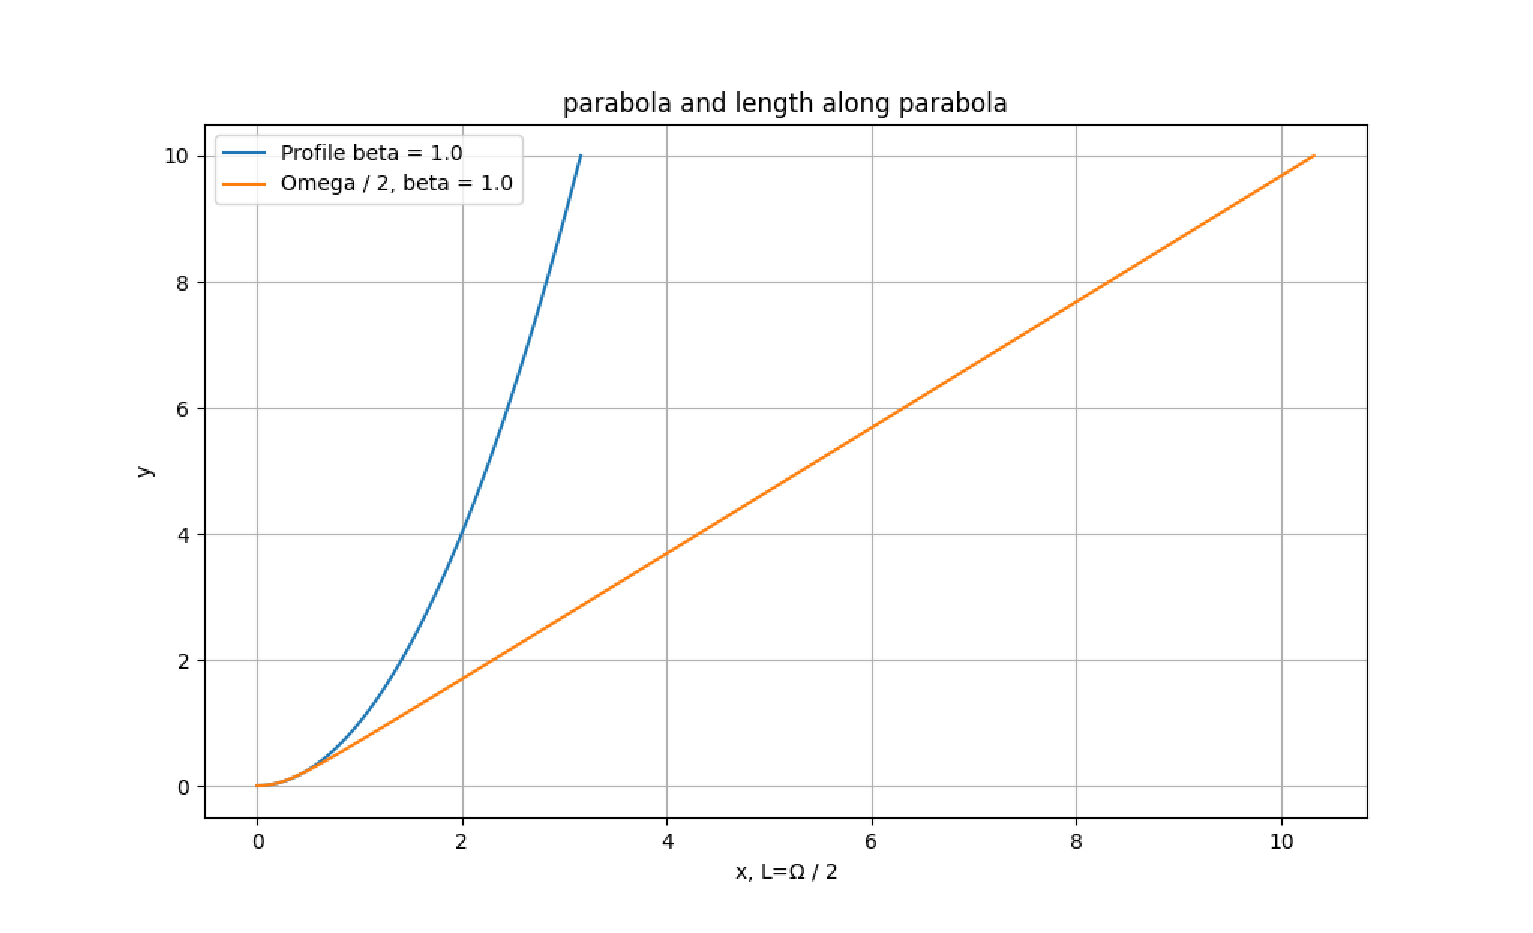
\includegraphics[width=0.8\textwidth]{/Users/Theo/Entiteiten/Hygea/2022-AGT/jupyter/images/parabola_omega}

\caption{\label{fig:Paraboolvormig-slootprofiel}Paraboolvormig slootprofiel
met halve omtrek $\Omega/$2. De have omtrek moet een rechte line
worden evenwijdig aan $x=y$ en voor zeer kleine $y$ samenvallen
met $x=y$.}

\end{figure}


\subsection{Elimineren van de slootwaterstand $h$ uit de vergelijking van de
lek}

Op dezelfde wijze als hiervoor is gedaan bij de wiskundig opgelegde
drainageweerstand, kan bij de fysieke weerstand het variabele slootpeil
uit het model worden gëelimineerd. Merk daarbij op dat het wiskundige
verband tussen slootdiepte en afvoer $y=\eta\sqrt{q}$ ongewijzigd
blijft

\begin{align*}
q & =\frac{\phi-h}{c_{dr}}=\frac{1}{c_{dr}}\left(\phi-h_{0}-y\right)=\frac{1}{c_{dr}}\left(\phi-h_{0}-\eta\sqrt{q}\right)
\end{align*}
zodat

\begin{align*}
q & =\frac{1}{c}\left(\phi-h_{0}-\eta\sqrt{q}\right)\\
q & =\frac{\phi-h_{0}}{c_{dr}+\frac{\eta}{\sqrt{q}}}
\end{align*}

Waarin de oorspronkelijke drainageweerstand $c_{dr}$ is uitgebreid
met de term $\frac{\eta}{\sqrt{q}}$.

Uiteraard is de weerstand $c_{dr}+\frac{\eta}{\sqrt{q}}$ nu een functie
van de slootdiepte. Echter in een externe rekencyclus wordt de lek
$q$ in elke cyclus herberekend, waardoor uiteindelijk de juiste oplossing
wordt verkregen. Het is essentieel dat tenminste de $q$ in de noemer
$\ge0$ blijft, ook al wordt $\phi<h_{0}$, net zoals dat bij vrije
drainage ook in werkelijkheid het geval is. Voor de drainageweerstand
geldt, eveneens om fysische redenen, dat zijn reciproke waarde $\ge$0
moet blijven. De wijze waarop $q$ positief gehouden wordt is hiervoor
beschreven; de wijze waarop $c_{dr}$ positief wordt gehouden voor
$\phi\le h_{0}$ (dit is $y<0)$ wordt hierna beschreven.

Hiermee zijn alle gegevens nodig voor een model met vrije afwatering
bekend.

\subsection{Voorkom dat $\Omega$ nul wordt wanneer $y<0.$}

Omwille van de convergentie van de oplossing van het op te stellen
stelsel vergelijkingen, is het essentieel dat dat $c$ en $q$ over
het hele spectrum van $\phi$ continu en positief zijn, aangezien
zowel $\frac{1}{c}$ als $q$ beide verticaal zijn wanneer slootdiepte
$y\downarrow0$. Hoe te voorkomen dat de lek $q$ negatief kan worden
is hiervoor al beschreven. Ook de reciproke drainageweerstand moet
positief blijven, maar wel praktisch nul voor $\phi<h_{0}$. $\Omega$
bestaat niet voor $\phi<h_{0}$ (negatieve slootdieptes) en is dus
dus niet continu bij $y\downarrow0$. We kunnen dit verhelpen door
$\Omega$ bij zeer kleine en negatieve $y$ over te laten gaan in
een functie die steeds net positief blijft.

Zoals hiervoor reeds afgeleid geldt dat voor $y\downarrow0$ de functie
$L\left(y,\beta\right)=\frac{\Omega\left(y,\beta\right)}{2}$ voor
elke $\beta$ wordt benaderd door

\[
y\downarrow0\rightarrow L\left(y\right)\approx x
\]

Met $x$ de halve slootbreedte en $y$ de slootdiepte en een parabolisch
slootprofiel volgens

\[
x=\beta\sqrt{y}
\]

We willen de functie $L\left(y\right)\approx x=\beta\sqrt{y}$ voor
$y<\hat{y}$, met $\hat{y}$ een kleine positieve waarde, continu
laten overlopen in een functie die met afnemende $y$ snel verwaarloosbaar
klein wordt maar wel positief blijft. Een geschikte functie hiervoor
is

\[
x=\delta e^{+\frac{y}{\lambda}}
\]

Deze functie zegt dat $x=\delta$ voor $y=0$ en exponentieel kleiner
wordt naarmate $y$ verder negatief wordt. De noemer $\lambda$ bepaalt
hoe snel dit gaat. In de praktijk kan voor $\delta$ een waarde van
bijvoorbeeld $\delta=0.01$ m of kleiner worden gekozen. De waarde
van $\lambda$ volgt uit die van $\delta$ vanuit de eis dat de functie
$\Omega$ en zijn afgeleide continu zijn op het punt $\hat{y}$, waarna
we $\Omega$ over het hele spectrum van $y$ kunnen berekenen, negatief
of niet.

Continuïteit voor het slootprofiel en de functie voor $y<\hat{y}$
vereist op het punt $y=\hat{y}$ dat zowel de functies als hun afgeleiden
aan elkaar gelijk zijn. Dus geldt

\begin{align*}
\beta\sqrt{\hat{y}} & =\delta e^{\frac{\hat{y}}{\lambda}}\\
\frac{\beta}{2\sqrt{\hat{y}}} & =\frac{\delta}{\lambda}e^{\frac{\hat{y}}{\lambda}}
\end{align*}

Beide vergelijkingen op elkaar delen elimineert $\delta$ en geeft
het transitiepunt $\hat{y}$ als een functie van $\lambda$

\[
\hat{y}=\frac{\lambda}{2}\,\,\,\leftarrow\rightarrow\,\,\,\lambda=2\hat{y}
\]

Vul in $\hat{y}=\frac{\lambda}{2}$ om $\delta$ te berekenen

\[
\beta\sqrt{\frac{\lambda}{2}}=\delta e^{\frac{1}{2}}\,\,\,\leftarrow\rightarrow\,\,\,\delta=\frac{\beta}{e^{0.5}}\sqrt{\frac{\lambda}{2}}\approx0.61\times\beta\sqrt{\frac{\lambda}{2}}
\]

We hebben nu, na keuze van $\hat{y}$

\begin{align*}
\lambda & =2\hat{y}\\
\delta & =0.61\times\beta\sqrt{\hat{y}}
\end{align*}

Kiezen we $\delta$, de ,,halve slootbreedte'' voor $y=0$ dan volgt

\[
\hat{y}=e\times\left(\frac{\delta}{\beta}\right)^{2}\approx2.72\times\left(\frac{\delta}{\beta}\right)^{2}
\]

Bijvoorbeeld $\hat{y}=0.01\,m$, waar dan uit volgt dat $\lambda=2\hat{y}=0.02\,m$
en met bijvoorbeeld $\beta=1$ volgt dan $\delta=0.6\sqrt{0.01}=0.06\,m$.
Merk op dat $\delta$ nu de ,,halve slootbreedte'' is en dus ook
de halve slootomtrek voor $y=0$. Dit lijkt een prima grootte voor
in het grondwatermodel. Eventueel kiezen we $\hat{y}=0.001$ of $\hat{y}=0.0001$.
Een waarde van $\lambda=0.02\,m$ impliceert dat $x$ voor $y=-5\lambda=-0.1\,m$
nog slechts $e^{-5}\delta\approx0.006\,\delta\approx4\times10^{4}\,m$
is, en dus volstrekt verwaarloosbaar. Merk op dat voor $y<\hat{y}$
geldt dat $L\left(y\right)\approx x=\delta e^{\frac{y}{\lambda}}$
en dat $\Omega=2L\left(y\right)$.

\newpage{}

\part{Implementatie in Fdm3}

\section{Intro}

Fdm3 is een stationair (intern tijdsafankelijk) eindig differentie
model, ,,Fdm3'', waarmee vlakke en axiaal-symmetrische doorsneden,
evenals volledig 3D eindige differentiemodellen kunnen worden opgezet.
Een eindig differentie model als Modflow of in dit geval Fdm3, berekent
de volumestroom $Q_{cel}$ {[}m$^{3}$/d{]} als volgt

\[
Q_{lek,cel}=C\left(h-\phi\right)=A\frac{h-\phi}{c}
\]

Hierin is $C$ {[}L2/T{]} de zogenoemde conductance (in Modflow jargon)
verder conductantie genoemd, $h$ de gefixeerde stijghoogte buiten
het model (slootpeil bijv.), dit is het zogenaamde drainagepeil, en
$\phi$ de berekende stijghoogte in het model. $A$ het oppervlak
van de rekencel en $c$ {[}T{]} de vlakdekkende weerstand van deze
rekencel tegen verticale grondwaterstroming. We zien dus dat $Q$
in het model positief is bij infiltratie en negatief bij lek.

De conductantie $C$ {[}m$^{2}$/d{]} die in het model wordt gebruikt
is dus

\[
C=\frac{A}{c}
\]

In de situatie met vrije afwatering is de drainagebasis $h$ afhankelijk
van de lek zelf. Omdat bij lek $Q<0$ is, geldt qua teken

\[
h=h_{0}+\eta\sqrt{q},\,\,\,q=\frac{-Q}{A}\ge0
\]

De drainagebasis $h$ is onbepaald (niet bestaand) voor $q<0$., dus
bij infiltratie. Inderdaad is $h$ dan volkomen onbepaald, aangezien
bij vrije drainage infiltratie fysisch niet kan optreden; de sloten
dan dan immers droog. De weerstand $c$ is hiervoor al uitgebreid
behandeld en kan dus direct worden gebruikt in het eindige differentie
model in de uitdrukking $C=A/c$.

De berekening van de stijghoogten moet iteratief gebeuren omdat de
weerstand afhangt van de te berekenen stijghoogte zelf. Deze iteratieve
berekening vindt plaats een zgnaamde rekenlus ,,outer loop'' waarin
steeds opnieuw de stijghoogten worden herberekend en waarna telkens
de weerstanden worden aangepast totdat de weerstanden en stijghoogten
niet meer veranderen.

\section{Stabilteit van het rekenproces}

Door de niet-lineariteit van de (drainage)weerstanden moet het stelsel
vergelijkingen binnen het eindige differentie model iteratief worden
opgelost in een zogenaamde rekenlus ,,outer loop'' waarbinnen telkens
de stijghoogten worden berekend, waarna de (drainage)weerstanden steeds
opnieuw worden aangepast, totdat convergentie is verkregen. Het op
deze manier bereiken van convergentie is echter hoogst onzeker. Dit
is in het algemeen zo bij niet-lineaire systemen, maar hier in het
bijzonder omdat een stationaire oplossing alleen mogelijk is wanneer
de stijghoogte in minstens een van de rekencellen direct of indirect
wordt vastgehouden. Hieraan wordt niet voldaan bij drainage wanneer
alle stijghoogten lager zijn dan het drainageniveau. Bovendien kunnen
de conductanties van de drain-cellen tussen opeenvolgende rekenlussen
 op een neer blijven springen, waardoor er ook om deze reden in een
aantal situaties nooit convergentie optreedt. Dit op een neer springen
van de drainageweerstand tussen opeenvolgende rekenlussen is op te
lossen door de overgang tussen wel drainage en geen drainage geleidelijk
te laten verlopen. Dit kan door de conductanties te vermenigvuldigen
met een sigmoïde functie die snel naar 1 gaat voor $\phi>h$ en snel
naar nul gaat voor $\phi<h$. Zo'n functie is

\[
y=\frac{1}{1+\exp\left(-y/\lambda\right)}
\]

Met $\lambda$ een klein getal, dat kan worden opgevat als de breedte
van de overgangszone. In het model wordt $\lambda=0.05$ m aangehouden.
Dit is geschikt vanuit praktijkoogmerk en blijkt in het model heel
goed te werken.

Het fundamentele probleem met de convergentie, namelijk ontbreken
van vaste randen bij het berekenen van een stationaire oplossing,
moeten we echter anders oplossen. Vanuit het besef dat er altijd een
niet-stationaire oplossing bestaat, kunnen we het model ook niet-stationair
doorrekenen. Bij een niet-stationaire berekening is er altijd een
beginvoorwaarde, oftewel een stijghoogteveld van waaraf wordt gestart.
Doordat er bij niet-stationaire oplossingen altijd berging is, blijft
de oplossing na een kleine tijdstap stabiel en nog dicht in de buurt
van de beginvoorwaarde. Door de tijdstap in elke volgende loop-cyclus
met een gegeven factor te vergroten, wandelt het model met steeds
grotere stappen door de tijd heen en bereikt zo altijd een stabiele,
stationaire eindwaarde. Deze eindwaarde is stabiel (stationair) mits
er uiteindelijk in het model cellen aanwezig zijn die de stijghoogte
direct of indirect via drains of vrije drainage vasthouden. Dat is
bij vrije drainage altijd het geval, omdat een model met vrije drainage
kan alleen zinvol kan zijn bij neerslag of permanente aanvoer, waardoor
initieel te lage grondwaterstanden gedurende de iteratiestappen stijgen
totdat de drainage aanslaat en stijghoogten in een deel van het model
alsnog worden gefixeerd. Hiermee is het convergentieprobleem fundamenteel
opgelost. We rekenen dus feitelijk niet-stationair ons stationair-bedoelde
model door, met niet-lineaire randvoorwaarden die over een korte hoogte
soepel overgaan naar nul, zonder die nul ooit te bereiken. De keuze
van de begintijdstap en de vermenigvuldigingsfactor is aan de gebruiker.
De keuze van de hoogte waarover de randvoorwaarden overgaan naar praktisch
nul, is nu vastgezet op 0.05 m, maar kan gemakkelijk worden aangepast.

Het is duidelijk dat dit model zeer gemakkelijk niet-stationair te
maken is, immers alle daartoe benodigde infrastructuur is er reeds
in geïmplementeerd en wordt bij de berekening van de stationaire eindsituatie
ook steeds gebruikt.

\section{Andere niet-lineaire randvoorwaarden}

In het eindige differentie model zijn naast de besproken vrije drainage
(FDR) ook andere randvoorwaarden geïmplementeerd, die overeenkomen
met die in Modflow. Dit zijn: GHB (general head boundaries), DRN (drains)
en RIV (rivers).

In geval van GHB-cellen zijn de conductanties constant zodat het model
net zo makkelijk kan infiltreren als kan lekken. GHB-randvoorwaarden
vergen geen rekenlus.

DRN-cellen kunnen lekken maar niet infiltreren. Deze randvoorwaarde
is niet-lineair en vergt wel een rekenlus waarin het stelsel van vergelijkingen
herhaald moet worden opgelost na bijstellen van paramaters. Bovendien
wordt ervoor gezorgd dat de overgang tussen ,,aan'' ($\phi>h$)
en ,,uit'' ($\phi<h$) geleidelijk verloopt over een hoogte van
ca 10 cm ($\lambda=0.05\,m)$.

RIV-cellen kunnen lekken en infiltreren zolang de stijghoogte zich
boven de bodem van de river ($r_{bot}$) bevindt. Daaronder blijft
de infiltratie constant en gelijk aan de conductantie maal de rivierdiepte.
Door de rivierstand even hoog in te stellen als de hoogte van de rivierbodem,
$h=r_{bot}$, werken RIV-cellen exact hetzelfde als DRN-cellen. Bij
RIV-cellen wordt de overgang $\phi>r_{bot}$ en $\phi<r_{bot}$ geleidelijk
gemaakt over een hoogte van ca 10 cm.

Met dit model is het derhalve gemakkelijk om de werking van verschillende
soorten randvoorwaarden te laten zien.

\section{Verkrijgen van de parameters nodig voor de simuatie van vrije drainage}

De vraag is nu hoe de parameters zijn te verkrijgen die nodig zijn
voor de simulatie van een gebied met vrije drainage. De meest praktische
aanpak is om uit te gaan van bekende gegevens in gemiddelde omstandigheden,
die als referentie geldt. Dat wil zeggen de grondwaterstijghoogte
$\phi_{N}$, de slootwaterstand (het drainageniveau) $h_{N}$ en de
slootbodemhoogte $h_{0}$ en dit samen met de gemiddelde gebiedsafvoer,
die meestal gelijk zal zijn aan het neerslagoverschot $N$. Bij gebruik
van de fysische drainageformule, hebben we nog de slootbreedte $w$
nodig voor de gemiddelde omstandigheden, en, tenslotte, de gemiddelde
slootafstand $L$. Ook hebben we de daarvoor de horizontale en verticale
doorlatendheid van het watervoerend pakket nodig. Deze zijn echter
in de invoer van het grondwatermodel aanwezig. Hiermee liggen alle
voor de simulatie van vrije drainage benodigde gegevens vast, en kunnen
de parameters worden bepaald die nodig zijn om de drainageweerstand
en het slootpeil te berekenen als functie van de afvoer. Deze parameters
zijn $\gamma$ en $\eta$.

Samenvattend: wat hebben we nodig om deze vorm van vrije afwatering
in het model te kunnen handelen?
\begin{enumerate}
\item $\phi_{N}$ de stijghoogte voorafgaand aan de ingreep behorend bij
gemiddelde neerslagoverschot $N$ rond dit modelknooppunt.
\item $h_{N}$ de slootwaterstand (drainagebasis) bij de slootafvoer behorend
bij het gemiddelde neerslagoverschot $N$ in het modelknooppunt.
\item $h_{0}$ de bodemhoogte van de sloten behorend tot het model knooppunt.
\item $N$ het gemiddelde neerslagoverschot (eventueel plus kwel) dat de
sloten uiteindelijk in de referentiesituatie afvoeren, dat wil zeggen
dat zijn afvoeren voorafgaand aan de te modelleren ingreep.
\item $w_{N}$ de gemiddelde slootbreedte behorend bij slootwaterstand $h_{N}$
\item $L$ de gemiddelde slootafstand.
\item $k_{x}$, $k_{z}$, direct afkomstig uit de invoer van het model.
\end{enumerate}
Items 5 t/m 7 zijn alleen nodig indien we de drainageweerstand fysisch
willen berekenen op basis van het slootprofiel in niet via de direct
opgegeven wiskundige relatie. Items 5 en 7 zijn dan ook optioneel.
Bevat de invoer de gegevens $w$ en $L$ dan rekent het model met
de fysische drainageweerstand op basis van een parabolisch slootprofiel.
Bij afwezigheid, rekent het model met de wiskundig opgelegde relatie
tussen afvoer en drainageweerstand.

Met deze gegevens kunnen we de verschillende coëfficiënten als volgt
berekenen.

De drainageweerstand in de referentiesituatie:

\[
c_{N}=\frac{\phi_{N}-h_{N}}{N}
\]
De coëfficiënt $\gamma$ waar we vervolgens de drainageweerstand wiskundig
kunnen uitrekenen als functie van de actuele afvoer:

\[
\gamma=c_{N}\sqrt{N}
\]
De coëfficiënt $\eta$ waarmee de slootdiepte kan worden berekend
als functie van de actuele afvoer:

\[
\eta=\frac{h_{N}-h_{0}}{\sqrt{N}}
\]

Wanneer we $c_{N}$ fysisch willen berekenen met natte omtrek $\Omega$
gebruiken we een parabolisch slootprofiel met $x$ de halve slootbreedte
en $y$ de slootdiepte volgens

\[
x=\beta\sqrt{y}
\]
Met gegeven halve breedte $b_{N}$ of hele slootbreedte $w_{N}=2b_{N}$
bij slootpeil $h_{N}$ volgt hiermee de relatie

\[
b_{N}=\beta\sqrt{h_{N}-h_{0}}
\]
waaruit de coëfficiënt $\beta$ kan worden berekend

\[
\beta=\frac{b_{N}}{\sqrt{h_{N}-h_{0}}}
\]


\section{Implementatie van vrije afwatering in Modflow}

Hiervoor is afgeleid dat voor het verband tussen slootdiepte en afvoer
volgens

\[
y=\eta\sqrt{q}
\]

en voor het verband tussen weerstand en afvoer

\[
\frac{1}{c_{dr}}=\frac{\sqrt{q}}{\gamma}
\]

de volgende afvoer relatie ontstaat, waaruit de slootdiepte $h$ is
geëlimineerd ten gunste van de bodemhoogte van de sloten $h_{0}$.
De afvoer is dan gegeven door

\[
q=\frac{\phi-h_{0}}{\left(\gamma+\eta\right)^{2}}\left(\phi-h_{0}\right)
\]

Wat impliceert dat de coëfficiënt voor de factor $\phi-h_{0}$ de
rol speelt van reciproke weerstand, of Modflow-termen als specifieke
conductantie $C_{s}$, die alleen nog met het celoppervlak moet worden
vermenigvuldigd om de typische Modflow conductantie te krijgen

\[
C_{s}=\frac{1}{c}=\frac{\phi-h_{0}}{\left(\gamma+\eta\right)^{2}}
\]

Deze uitdrukking geeft weer dat bij de getroffen aannamen over de
slootdiepte en weerstand als functie van de afvoer, de specifieke
conductantie evenredig is met de stijghoogte boven de slootbodem.
Aangezien we de weerstand in de referentiesituatie kennen, namelijk
die waarbij de afvoer gelijk is aan het neerslagoverschot $q=N$,
met bijbehorende stijghoogte $\phi_{N}$ evenals de hoogte van de
slootbodem $h_{0}$ kan nu de specifieke conductantie direct worden
gegeven als lineaire functie van de grondwaterstand boven het slootpeil.
We hebben daarvoor de $\gamma$ en de $\eta$ helemaal niet nodig.
Wat we nodig hebben is de specifieke conductantie in de referentiesituatie

\[
C_{s_{N}}\left(\phi_{N}-h_{0}\right)=\frac{\phi_{N}-h_{0}}{\left(\gamma+\eta\right)^{2}}\left(\phi_{N}-h_{0}\right)=N
\]

Waarbij de middelste uitdrukking overbodig is, zodat

\[
C_{s_{N}}=\frac{N}{\phi_{N}-h_{0}}
\]

Verder geldt dat $C_{s}=0$ voor $\phi_{n}\le h_{0}$ en verloopt
$C_{s}$ linear tussen $\phi=h_{0}$ en $\phi=\phi_{N}$.

In een model als Modflow kunnen we lek boven een gegeven niveau berekenen
met de optie DRN. Cellen met de DRN optie krijgen een drainniveau
$h_{0}$ mee waarboven lek mogelijk is. En hierbij hoort een vaste
conductantie. We kunnen echter in elke cel van Modflow een willekeurig
aantal DRNs tegelijk opleggen, elk met een eigen drainniveau en een
eigen conductantie. Op deze wijze kunnen we de conductanties in een
rekencel stapelen met als resultaat een cel waarvan de netto of per
saldo DRN-conductantie verloopt met de grondwaterstand. Op deze wijzen
kan elk gewenst verband tussen de per saldo conductantie en de grondwaterstand
worden gerealiseerd. Wanneer we dicht bij de afleiding willen blijven
zullen we de conductantie lineair met de grondwaterstand willen laten
toenemen. Maar dat hoeft duidelijk niet.

De grootte van de gestapelde specifieke conductantie als functie van
de grondwaterstand $\phi$ is zo

\[
C_{\phi}=\sum_{i}C_{i,\phi>h_{i}}
\]

Waar $C_{i}$ de specifieke conductantie die geldt bij $\phi>h_{i}$,
het drainniveau van specifieke conductantie $i$.

Het verband tussen grondwaterstand en afvoer wordt

\[
q_{\phi}=\sum_{i}\left\{ C_{i}\left(\phi-h_{i}\right),\phi>h_{i}\right\} 
\]

Dit is dus een niet-lineaire grondwaterstandafvoerrelatie. Terwijl
de standaard DRN optie, met een DRN per cel een lineaire grondwaterstandafvoerrelatie
vertegenwoordigt

\[
q_{\phi}=C_{s,dr}\left(\phi-h\right)=\frac{1}{c_{dr}}\left(\phi-h\right)
\]

Waarbij normaliter het slootpeil $h$ of de drainagebasis wordt gebruikt
met vast peil $h$, maar in geval van vrije afwatering

\[
q_{\phi}=C_{s}\left(\phi-h_{0}\right)
\]

waarbij $C_{s}<C_{s,dr}$ omdat $\phi-h<\phi-h_{0}$.

We kunnen nu de (specifieke) conductantie in $n$ stapjes laten toenemen
boven de slootbodemhoogte $h_{0}$. De eis daarbij is dat de afvoer
$q=N$, het neerslagoverschot in de referentiesituatie, dus bij $\phi=\phi_{N}$

\[
q=N=\sum_{i}^{n}C_{i}\left(\phi_{N}-h_{i}\right)=C\left(\phi_{N}-h_{0}\right)
\]

Wanneer de stapjes $C_{i}$ alle gelijk zijn dan krijgen we

\[
C_{i}\left(n\phi_{N}-\sum_{i}^{n}h_{i}\right)=C\left(\phi_{N}-h_{0}\right)
\]

zodat

\[
C_{i}=\frac{C}{n}\times\frac{\phi_{N}-h_{0}}{\phi_{N}-\overline{h_{i}}}
\]

met $\overline{h_{i}}$ het gemiddelde van de staphoogtes van de drainstapjes.
De laatste factor brengt dus in rekening dat de verschillende drains
een verschillend drainniveau hebben waarboven zij pas gaan afvoeren.

Figuur \ref{fig:Conductantie-vs-phi} laat voor verschillend aantal
drainniveau's de cumulatieve conductantie zien, waarvan de stapjes
voldoen aan bovenstaande vergelijking. De rode punt geeft de situatie
met slechts één stap en de referentiestijghoogte $\phi_{N}$ die ook
in de volgende figuur staat.

\begin{figure}[h]
\centering
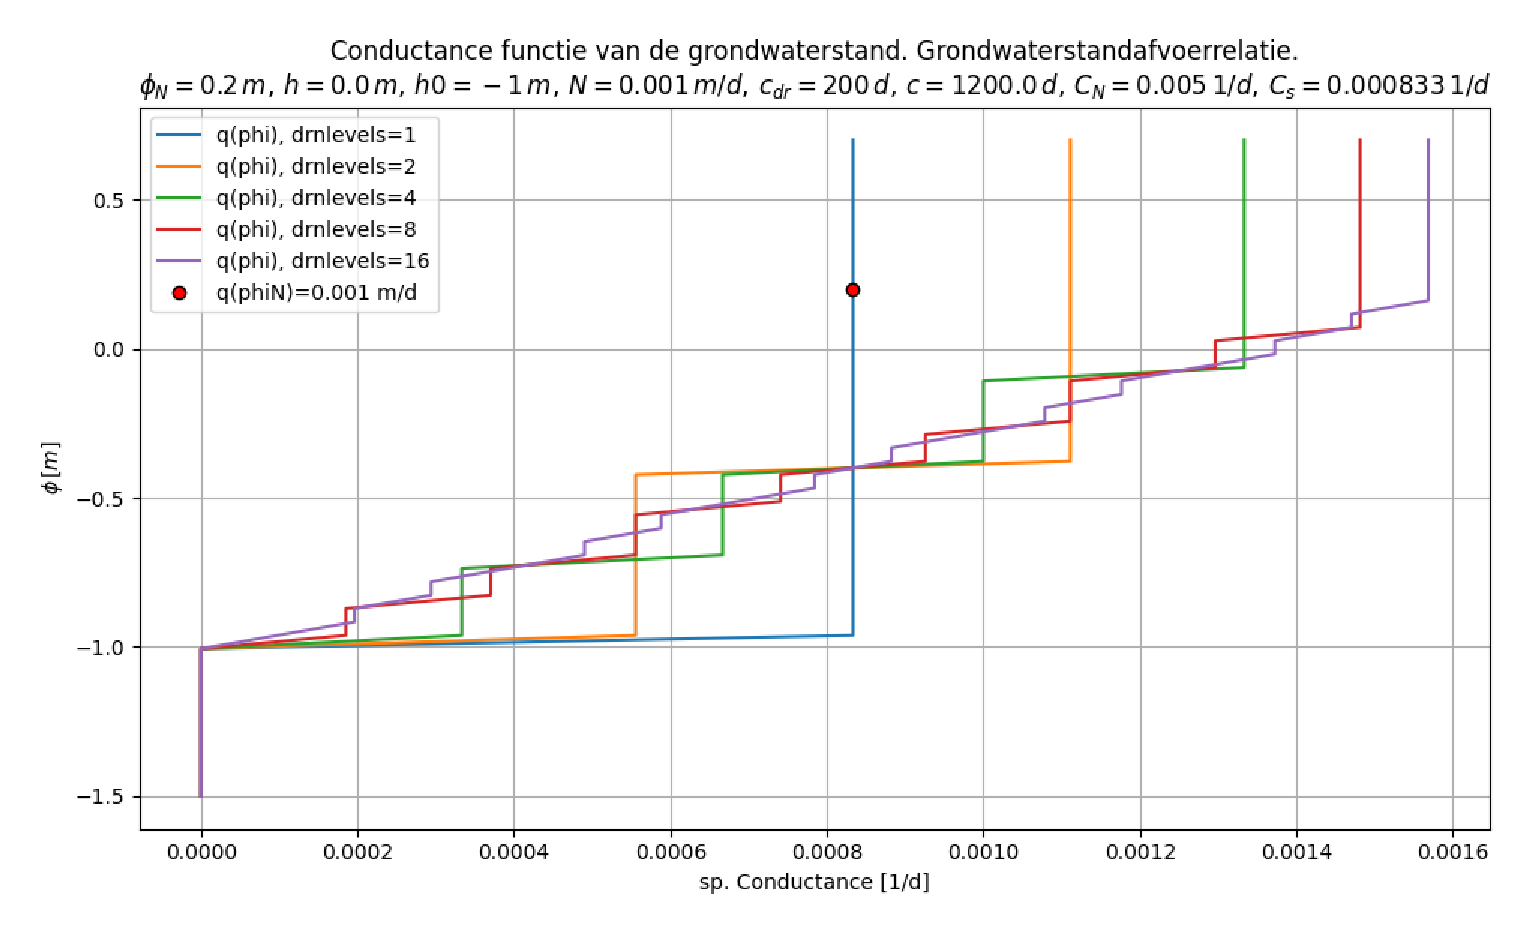
\includegraphics[width=0.8\textwidth]{/Users/Theo/Entiteiten/Hygea/2022-AGT/jupyter/images/plt_test}

\caption{\label{fig:Conductantie-vs-phi}Conductantie als functie van de grondwaterstand
bij verschillend aantal drainageniveau's}

\end{figure}

Figuur \ref{fig:Afvoer-vs-phi} toont de lek (afvoer) als functie
van de grondwaterstand bij een verschillend aantal drainageniveau's.
De conductantie van de drainagestappen is berekend met bovenstaande
formule zodanig dat de afvoer bij de referentiegrondwaterstand $\phi_{N}$
gelijk is aan het neerslagoverschot $N$. Dit punt is aangegeven met
de rode stip waar alle lijnen inderdaad doorheen gaan.

\begin{figure}[h]
\centering
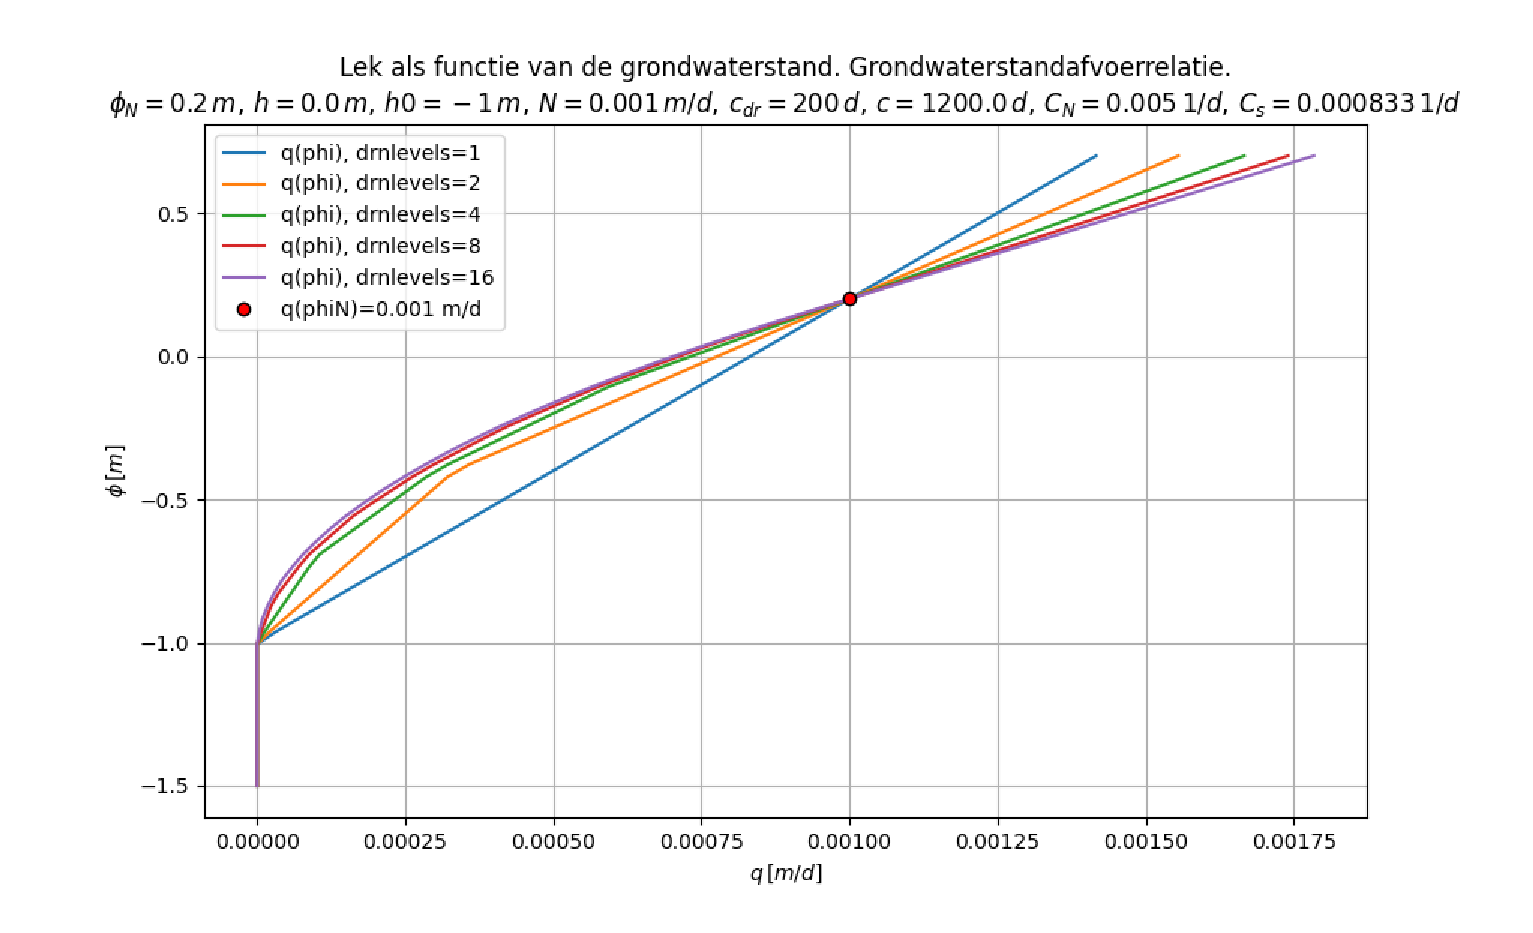
\includegraphics[width=0.8\textwidth]{/Users/Theo/Entiteiten/Hygea/2022-AGT/jupyter/images/lek_vs_phi_drn1}

\caption{\label{fig:Afvoer-vs-phi}Afvoer als functie van de grondwaterstand
bij een verschillend aantal drainageniveau's.}

\end{figure}

Figuur \ref{fig:Afvoer-vs-phi} geeft dus in feite de grondwaterstandafvoerrelatie
voor verschillend aantal drainageniveau's. Bij een enkel niveau is
dit verband lineair. Maar met toenemend aantal komt de relatie steeds
beter overeen met de oorspronkelijk aangenomen vorm van de weerstand,
$q=\left(\frac{\phi-h_{0}}{\gamma+\eta}\right)^{2}$ of $\phi-h=\left(\gamma+\eta\right)\sqrt{q}$
met $\gamma+\eta$ een constante die in de afleiding hiervoor niet
meer nodig is omdat de conductantiestappen zijn afgeleid van de weerstand
in de referentiesituatie. Voor grotere waarden van $q$ bevindt is
het verband tussen $\phi$ en $q$ lineair omdat daar geen verdere
drainageniveau's meer zijn gedefinieerd. Maar dat zou natuurlijk wel
kunnen.

We kunnen natuurlijk hele discussies gaan voeren over de vraag of
het verband tussen de conductantie en $\sqrt{q}$ danwel het verband
tussen het (geëlimineerde) slootpeil en $\sqrt{q}$ adequaat zijn,
maar dat levert uiteindelijk weinig verschil op in de uitkomst. Het
hier verkregen resultaat is zeer praktisch: de conductantie neemt
lineair toe met de grondwaterstand boven het basis slootniveau. Dit
is gemakkelijk in Modflow toe te passen. Maar natuurlijk staat het
de gebruiker toe om elk ander verband middels meervoudige drainages
in rekencellen te verwezenlijken, bijvoorbeeld op basis van verschillende
typen sloten die in een gebied voorkomen. Ik verwacht echter weinig
wezenlijk verschil omdat bij vrije drainage voor elk type sloot een
lineair verband moet worden verwacht tussen conductantie en grondwaterstand,
zodat dat ook mag worden verwacht bij representatie van het voorkomen
van sloten van verschillende categoriëen, wanneer die alle voldoen
aan vrije afwatering. Tenslotte, het staat ieder vrij om in dergelijke
situaties de drainniveau's voor het representeren van vrije drainage
te mengen met standaard Modflow drains die sloten modelleren met een
vast peil in hetzelfde gebied. Het zijn tenslotte alle standaard drain-opties
die worden toegepast, hoeveel dat er per rekencel zijn is om het even.

Hieraan mag worden toegevoegd dat wat hier geldt voor drains op vergelijkbare
wijze van toepassing is op de RIV (rivier) optie. Ook daarvan kan
men vele aan een enkele cel opgeven om een groot aantal waterlopen
tegelijk te simuleren. En natuurlijk geldt hetzelfde voor de algemene
GHB (general head) optie, de enige lineaire optie die geen buiteniteraties
nodig heeft.

Figuur \ref{fig:lek-per-drnlevel} geeft de berekende lek langs de
lengte van het model. De groene lijn ,,q DRN'' is berekend met de
standaard DRN optie waarbij de drainage wegvalt zodat de grondwaterstand
zakt beneden het oorspronkelijke slootniveau $h$, geheel onafhankelijk
van de slootdiepte. De paarse lijn met de puntjes is de lek wanneer
de conductantie vanaf de slootbodem in 6 stapjes toeneemt tot $h_{i}=1.0$
m, net onder de grondwaterstand in de referentiesituatie $\phi=0.2$
m. De totale lek, dus het oppervlak onder beide grafieken is dezelfde
(het totale neerslagoverschot op het model minus de onttrekking die
een kwart daarvan is). Elk van de gekleurde lijnen onder in de grafiek
geeft de lek van een afzonderlijk drainniveau. De grootste lek komt
van het laagste drainniveau en de kleinste lek van het hoogste drainniveau.
Opgeteld geven deze lijnen de paarse lijn met de puntjes.

\begin{figure}[h]
\centering
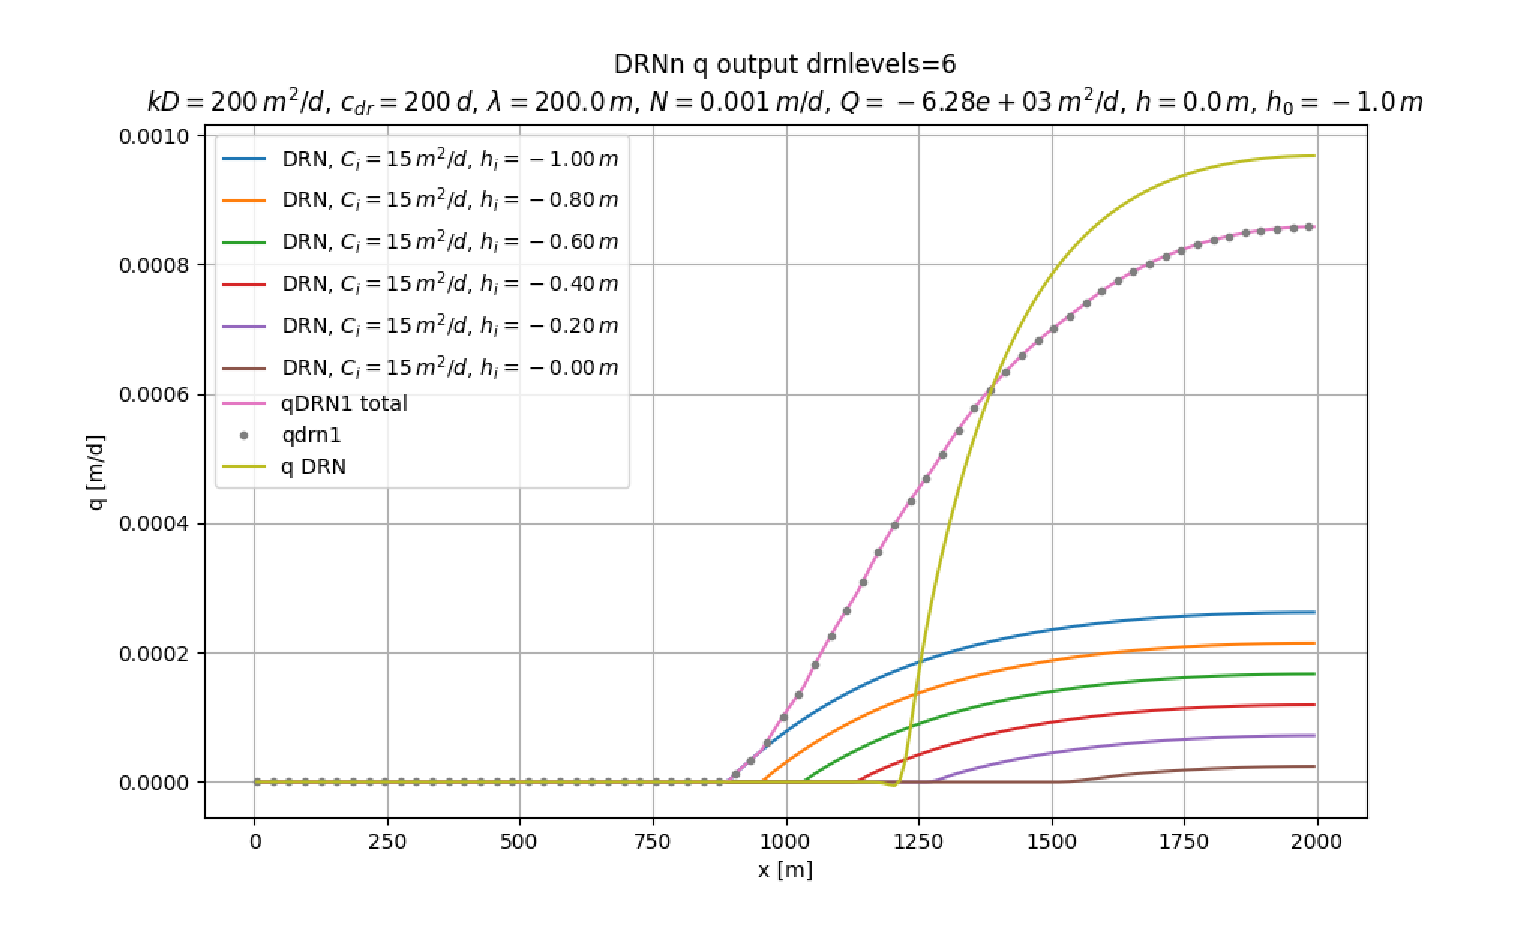
\includegraphics[width=0.8\textwidth]{/Users/Theo/Entiteiten/Hygea/2022-AGT/jupyter/images/DRNn_leakage}

\caption{\label{fig:lek-per-drnlevel}De lek met de standaard DRN optie en
met 6 verschillende drainageniveau's}

\end{figure}

\newpage{}

\part{Testen van het model}

\section{Vergelijking van modellen met verschillende randvoowaarden}

Met een en hetzelfde grondwatermodel hier Fdm3, kunnen verschillende
modellen worden opgezet die over en weer kunnen geverifieerd en ook
kunnen worden vergelijken met analytische oplossingen, althans voor
zover deze analytische oplossingen bestaan. Voor niet-lineaire grondwaterproblemen
bestaan die vaak niet. Met het oorspronkelijk in Matlab en de laatste
jaren in Python doorontwikkelde eindige differentie model kunnen stationaire
en tijdsafhankelijke modellen worden opgezet met een model netwerk
bestaande uit rechthoekige cellen en lagen waarvan de laagdikte variabel
is per cel. Dit is dezelfde opzet als bij oudere Modflow modellen.
Zo'n netwerk is relatief eenvoudig maar maakt het Python programma
van hoogstens een paar honderd regels code uiterst transparant. Fdm3
is verder uitermate geschikt voor het maken van doorsnedemodellen,
zowel vlakke als axiaal-symmetrische.

Voor het oplossen van het stelsel vergelijkingen wordt gebruik gemaakt
van de solvers uit de Scipy library, de beste ter wereld, waardoor
oplossing van het grondwatermodel geen probleem is, zolang het model
lineair is. Net als Modflow heeft het Python model, Fdm3, ook niet-lineaire
randvoorwaarden, namelijk DRN (drains), RIV (river) en FDR (vrije
drainage). De DRN cellen laten alleen water het model uit wanneer
de stijghoogte in de betreffende cel hoger is dan het opgegeven niveau
van de drain(s). Nooit kan er water via de DRN het model instromen.
De RIV-cellen laten water in- en uitstromen zolang de stijghoogte
van de RIV-cellen in het grondwatermodel is hoger dan het opgegeven
niveau van de rivierboden. Zakt de stijghoogte tot onder de rivierbodem
dan raakt de infiltratie via de rivierbodem los van de stijghoogte
het grondwater; zij wordt dan constant en gelijk aan de diepte van
de rivier gedeeld door de opgegeven weerstand van de rivierbodem.
Zowel DRN als RIV randvoorwaarden zijn niet-lineair en maken het grondwatermodel
dus ook niet-lineair. Fdm3 heeft nog een derde niet-lineaire randvoorwaarde,
namelijk die voor vrije ontwatering, FDR, waarin de drainageweerstand
afhankelijk is van de slootdiepte, dus van de waterstand in de sloot
minus de hoogte van de slootbodem. Bij vrije afwatering is geen infiltratie
mogelijk, net zoals bij de DRN-cellen; alleen is bij DRN-cellen de
uittreeweerstand constant terwijl die bij vrije ontwatering, FDR,
een functie is van de actuele slootdiepte. Daarnaast is ook de slootdiepte
zelf een functie is van de afvoer vanuit het model via de cellen met
vrije afwatering. De laatste vorm van afwatering sluit beter aan bij
de situatie in hogere of overgangsgebieden met een vrije afvoer, waar
geen extern water naartoe geleid of gepompt kan worden.

De afleiding voor de randvoorwaarden met vrije drainage is hiervoor
al gegeven. FDR komt in twee varianten
\begin{enumerate}
\item De drainageweerstand is een opgelegde wiskundige functie van de afvoer.
\item De drainageweerstand wordt berekend op basis van de actuele slootdiepte
en het slootprofiel, waarbij de slootdiepte afhankelijk is van de
afvoer.
\end{enumerate}
In dit hoofdstuk staat de verificatie van het model Fdm3 centraal
onder verschillende randvoorwaarden.

\section{Vlakke en axiaal symmetrische doorsnede modellen met verschillende
randvoorwaarden}

Het gemakkelijkst is de werking van de verschillende randvoorwaarden
te demonstreren aan de hand van vlakke of axiaal-symmetrische doorsnedemodellen.
De essentie hierbij is het zoveel mogelijk kunnen toetsen aan analytische
oplossingen en de modellen met verschillende randvoorwaarden onderling
te kunnen vergelijken en toetsen. 

We beginnen met vlakke eendimensionale modellen. Deze bestaan gemakshalve
steeds uit slechts een modellaag. We kunnen zo'n model bestaande uit
slechts een laag semi-gespannen maken door gebruik van de verschillende
randvoorwaarden GHB, DRN, RIV en of FDR. Zo kunnen we alle cellen
GHB cellen maken (general head boundaries). Door de zogenoemde conductantie
van de GHB-cellen equivalent te maken aan de weerstand van een scheidende
laag wordt de laag in feite semi-gespannen en wordt hetzelfde als
met een analytische oplossing voor een semi-gespannen grondwater.
Om de drainage te simuleren kiezen we een semi-gespannen laag waar
we direct het neerslagoverschot in injecteren. Hierdoor lekt water
via de scheidingslaag opwaarts. Verder leggen we een onttrekking $q_{0}$
{[}m2/d{]} op bij $x=0$. Hier door gaat water op korte afstand van
de onttrekking van de weerstandslaag infiltreren.

\section{Vergelijking tussen GHB- en DRN-randvoorwaarden}

Bij GHB randvoorwaarden kan water zowel infiltreren als exfiltreren;
bij DRN randvoorwaarden is alleen exfiltratie mogelijk. Het eenlaagsmodel
met GHB randvoorwaarden is gelijk aan een tweelaagsmodel met een vast
peil in de bovenste laag en tussen de twee lagen een weerstand biedende
laag. We laten hierna de resultaten zien van de simulatie in een vlak
1D doorsnedemodel en in een axiaal-symmetrisch doorsnede model. Deze
resultaten worden vergeleken met die van de analytische oplossing
voor hetzelfde probleem.

\subsection{De vlakke (1D) doorsnede}

De analytische oplossing voor deze situatie is die van Mazure plus
$Nc$

\[
\phi-h=q_{0}\frac{\lambda}{kD}e^{-\frac{x}{\lambda}}+Nc
\]

Met $q_{0}=\frac{kD}{\lambda}\left(\phi_{0}-h\right)$ en $N=0$ krijgen
we de bekende formule van Mazure, namelijk $\phi-h=\left(\phi_{0}-h\right)e^{-\frac{x}{\lambda}}$.
Met $q_{0}=0$ is de stijghoogte $\phi-h=Nc$ en uniform, dit is de
stijghoogte die nodig is om het neerslagoverschot $N$ via de weerstand
naar de omgeving te laten lekken. De weerstand $c$ moet hier worden
opgevat als drainageweerstand, dus de weerstand die het aanwezige
oppervlaktesysteem biedt tegen lek van grondwater. De stijghoogte
zal door het neerslagoverschot in een groot deel van het model boven
de drainagebasis $h$ liggen. In de buurt van de onttrekking zakt
de stijghoogte tot onder de drainagebasis. In de formule voor semi-gespannen
water en bij gebruik van GHB-cellen, treedt daar dan infiltratie op.
Bij gebruik van DRN-cellen wordt deze infiltratie afgekapt. Hierdoor
is de verlaging nabij de onttrekking bij gebruik van DRN cellen groter
dan bij GHB cellen als randvoorwaarde.

Figuur \ref{fig:Vlakke-dsn} geeft het resultaat van zowel de analytische
oplossingen en de simulatie met het Fdm3 model voor de vlakke (1D)
doorsnede. De analytische oplossing voor de situatie met semi-spanningswater
over de gehele $x$-as valt samen met die van de Fdm3-simulatie waarbij
GHB-randvoorwaarden zijn gebruikt, waardoor zowel lek als infiltratie
kan optreden. Dit is identiek aan een grondwaterpakket dat is afgedekt
door een slecht-doorlatende laag met daarboven een vast peil $h$
en waarin het neerslagoverschot direct wordt geïnjecteerd. De analytische
en de numerieke oplossing vallen over elkaar heen, zowel wat betreft
de stijghoogte als de lek.

Figuur \ref{fig:Vlakke-dsn} geeft hiernaast de analytische oplossing
volgens Blom samen met de numerieke waarbij voor de bovenrandvoorwaarde
in plaats van GHB-cellen DRN-cellen zijn toegepast. DRN-cellen laten
geen infiltratie toe. Bij Blom treedt lek op zolang de grondwaterstand
boven het slootpeil (de drainagebasis) blijft. De lek is daar een
deel van het neerslagoverschot de voeding is daar gelijk aan het neerslagoverschot
minus de lek. Binnen het gebied waar de de grondwaterstand onder de
drainagebasis zakt treedt geen lek meer op. De voeding is daar gelijk
aan het gehele neerslagoverschot. De afstand waarop de grondwater
is verlaagd tot de drainagebasis (verlaging is $Nc_{dr}$) is met
een zwarte verticale lijn aangeven. De analytische oplossing volgens
Blom is identiek aan de numerieke simulatie met DRN-cellen als bovenrandvoorwaarde
en het neerslagoverschot direct geïnjecteerd in de watervoerende laag.

De figuur met de lek en de voeding laat zien dat de lek voor $x<L$
nul is en daarbuiten evenredig met de verlaging. Voor de analytische
oplossing van Blom is de voeding weergegeven. Deze is voor $x<L$
gelijk aan het neerslagoverschot en neemt daarbuiten af tot nul voor
grote $x$. De som van de analytische voeding en de numeriek berekende
lek is gelijk aan het neerslagoverschot. De bovenste figuur laat ook
zien dat de verticale lijn het punt snijdt waar de grondwaterstand
is gezakt tot de drainagebasis $h=0$ vanaf de grondwaterstand zonder
onttrekking $\phi=h+Nc$.

\begin{figure}[h]
\centering
\includegraphics[width=0.8\textwidth]{/Users/Theo/Entiteiten/Hygea/2022-AGT/jupyter/images/example_fdm3_1D}

\caption{\label{fig:Vlakke-dsn}Analytische oplossingen en Fdm3-simulatie van
vlakke doorsnede. Het Fdm3-model bestaat uit een enkele modellaag.
Voor de gebruikte gegevens zie de kop van de bovenste figuur. Vergelijking
tussen de situaties met GHB- en met DRN-cellen. Boven de stijghoogten
en onder de lek respectievelijk de voeding van het pakket.}

\end{figure}


\subsection{De axiaal-symmetrische doorsnede}

Figuur \ref{fig:Ax-symm-dsn} geeft de resultaten berekende analytische
oplossing en de numerieke simulatie voor een axiaal-symmetrische doorsnede
met exact dezelfde gegevens als hiervoor gebruikt zijn bij de vlakke
doorsnede. Alleen de onttrekking heeft nu dimensie m$^{3}$/d in plaats
van m$^{2}$/d, maar is net als bij de vlakke doorsnede gelijk gesteld
aan de helft van het totale neerslagoverschot dat op het model valt.

\begin{figure}[h]
\centering
\includegraphics[width=0.8\textwidth]{/Users/Theo/Entiteiten/Hygea/2022-AGT/jupyter/images/example_fdm3_axsym}

\caption{\label{fig:Ax-symm-dsn}Analytische oplossingen en Fdm3-simulatie
van axiaal-symmetrische verticale doorsnede. Het Fdm3-model bestaat
uit een enkele modellaag. Voor de gebruikte gegevens zie de kop van
bovenste figuur. Vergelijking situatie met GHB- en DRN-cellen. Boven
de stijghoogten en onder de lek, respectievelijk de voeding van het
pakket.}

\end{figure}

De analytische oplossing voor de situatie met een onttrekking $Q_{0}$
{[}m$^{3}$/d{]} en met rechtstreeks injecteren van het neerslagoverschot
$N$ in het watervoerende pakket is dan

\[
\phi-h=\frac{Q_{0}}{2\pi kD}K_{0}\left(\frac{r}{\lambda}\right)+Nc
\]

$K_{0}\left(...\right)$ is uiteraard de bekende gemodificeerde Besselfunctie
en $\lambda$ als hiervoor. Zonder de injectie, dus met $N=0$ hebben
we de formule van De Glee en met $Q=0$ krijgen we net als hiervoor
een uniforme stijghoogte $\phi=h+Nc$, die nodig is om het geïnjecteerde
neerslagoverschot naar het oppervlaktewater te laten lekken via de
drainageweerstand $c_{dr}$. Ook deze formule berekent infiltratie
nabij de put, waar de stijghoogte tot onder het drainageniveau $h$
wordt getrokken. Hetzelfde krijgen we als we in het model GHB-randvoorwaarden
gebruiken. De analytische en de numeriek oplossingen blijken geheel
in overeenstemming, evenals de berekende lek/voeding die in de onderste
figuur is weergegeven. De voeding $n_{r}$ is natuurlijk $n_{r}=\frac{\phi_{r}-h}{c}$.

Bij gebruik van DRN-randvoorwaarden wordt deze infiltratie volledig
afgekapt. De verlaging is hierdoor groter bij gebruik van DRN-randvoorwaarden
dan bij GHB-randvoorwaarden. De analytische oplossing die volgens
\cite{Blom73} die geldt voor het gebied $r>R$ is de formule die
\cite{Glee30} voor semi-spanningswater afleidde. Die voor het gebied
met $r<R$ is de zogenaamde formule van Verruijt (dit is de formule
van Dupuit plus neerslagoverschot). De figuur laat zien dat de analytische
oplossing volgens Blom geheel overeenkomt met de numeriek oplossing
met DRN-cellen als bovenrandvoorwaarde. De grens tussen beide gebieden
is aangegeven met de verticale zwarte lijn. Dit is de straal waar
de stijghoogte is gedaald tot de drainagebasis $h$. De onderste figuur
met de lek/voeding laat zien dat de lek voor $r<R$ gelijk aan nul
is, maar de voeding gelijk aan het gehele neerslagoverschot. Op deze
grens is de verlaging gelijk aan $Nc_{dr}$ en is de voeding gelijk
aan $N$ en de lek gelijk aan nul.

Voor de verhouding tussen van voeding $n_{r}$ op afstand $r$ ten
opzichte van de voeding $n_{R}=N$ die op afstand $R$ geldt 

\[
n_{r}=N\frac{K_{0}\left(\frac{r}{\lambda}\right)}{K_{0}\left(\frac{R}{\lambda}\right)}
\]


\section{Simulatie met vrije afwatering of vrije drainage}

Hiervoor zagen we dat de analytische situatie volgens Blom identiek
is aan de numerieke simulatie met DRN-cellen als bovenrandvoorwaarde
en directe injectie in het watervoerende pakket. De situatie met vrije
afwatering lijkt hierop, maar verschilt in het feit dat daarbij de
drainagebasis (het slootpeil) lager wordt naarmate de lek afneemt
en het feit dat de drainageweerstand toeneemt met de afnemende slootdiepte.
Er kan alleen lek zijn zolang de grondwaterstand hoger is dan de slootbodem.
Zodra de grondwaterstand daaronder zakt is de lek nul en de drainageweerstand
dus oneindig groot. In een vrij afwaterend gebied is geen aanvoer
van water en geen infiltratie mogelijk. Dit is in de werkelijkheid
niet overal helemaal waar, omdat er natuurlijk water van bovenstrooms
naar de sloten kan lekken, dat vervolgens benendenstrooms weer infiltreert.
Zulke omstandigheden vallen buiten bestek van dit document en kunnen
alleen met een combinatie van een grond- en een oppervlaktewatermodel
enigszins zinvol worden gemodelleerd.

De drainageweerstand wordt gedefinieerd als

\[
c_{dr}=\frac{\phi-h}{N}
\]

Dat wil zeggen het verschil tussen de gemiddelde grondwaterstand met
het drainageniveau (het slootpeil) gedeeld door de gemiddelde drainage
(zonder kwel is dat gelijk aan het neerslagoverschot). In deze formule
zit ook het drainageniveau, dat echter bij vrije afwatering zelf afhang
van de lek. En daarmee is de drainageweerstand ook afhankelijk van
de actuele lek. In de theoretische afleidingen hebben we echter gezien
dat we ook de weerstand als volgt kunnen definiëren,

\[
c=\frac{\phi-h_{0}}{N}
\]
waarbij in plaats van de actuele maar variabele drainagebasis $h$
nu de vaste bodemhoogte van de sloten $h_{0}$ staat. De weerstand
$c$ is dan dus niet meer de drainageweerstand maar een andere, grotere.

\[
q=\frac{\phi-h_{0}}{c_{dr}+\frac{\eta}{\sqrt{q}}}\,\,\,\rightarrow c=c_{dr}+\frac{\eta}{\sqrt{q}}
\]

Hierin is de slootdiepte $y=h-h_{0}$ verwerkt waarvoor is gesteld
dat die via een eenvoudige functie van de lek $q$ afhangt

\[
y=\eta\sqrt{q}
\]
waarin de coëfficiënt $\eta$ volgt uit de slootdiepte in de referentiesituatie
wanneer $q=N$. De weerstand $c$ hangt nu zelf van de lek $q$ af.
Wanneer $q\downarrow0$ gaat $c\uparrow\infty$ en stopt de lek.

\subsection{De vlakke 1D doorsnede}

Figuur \ref{fig:Vlakke-dsn} geeft het resultaat voor de simulatie
van de vlakke doorsnede met GHB randvoorwaarde en de bijbehorende
analytische oplossing

\[
\phi=h+Nc-\frac{\lambda}{kD}Qe^{-\frac{x}{\lambda}},\,\,\,\lambda=\sqrt{kDc_{dr}}
\]

samen met het resultaat met DRN randvoowaarden en de daarbij behorende
analytische oplossing van Blom. Het resultaat met de GHB-randvoorwaarden
valt samen met de analytische oplossing en dat met de DRN-randvoorwaarde
valt samen met de analytische oplossing volgens Blom. De onderste
figuur geeft de bijbehorende lek. Die voor het model met de GHB-randvoorwaarde
slaat om in infiltratie zodra de grondwaterstand onder het (vaste)
slootpeil zakt, dat wil zeggen, zodra de verlaging groter is dan $Nc_{dr}$.
Die voor het model met de DRN-randvoorwaarde wordt nul zodra dit het
geval is. De grens waarbinnen de drains droogvallen is aangegeven
met de verticale lijn. De onderste figuur geeft ook de voeding van
het grondwater volgens Blom. Deze is nul waar de sloten het volledige
neerslagoverschot drains/sloten het volledige neerslagoverschot afvoeren
en is gelijk aan het neerslagoverschot waar de drains niets afvoeren.
De voeding plus lek is gelijk aan het neerslagoverschot.

\begin{figure}[h]
\centering
\includegraphics[width=0.8\textwidth]{/Users/Theo/Entiteiten/Hygea/2022-AGT/jupyter/images/example_fdm3_1D}

\caption{\label{fig:Vlakke-dsn+GHB+DRN}Analytische oplossingen en Fdm3-simulatie
voor GHB randvoorwaarden en voor DRN randvoorwaarden. De drains vallen
droog zodra de grondwaterstand onder het drainniveau daalt, dat hier
gelijk is aan het slootpeil. De verlaging is dan $Nc$. Boven de stijghoogten
en onder de lek en de voeding volgens Blom die overeenkomt met de
numerieke situatie met DRN randvoowaarden. Voeding volgens BLom plus
lek met DRN randvoorwaarden is gelijk aan het neerslagoverschot.}

\end{figure}

\begin{figure}[h]
\centering
\includegraphics[width=0.8\textwidth]{/Users/Theo/Entiteiten/Hygea/2022-AGT/jupyter/images/example_fdm3_1D+FDR}

\caption{\label{fig:Vlak-DRN+FDR}Analytische oplossingen en Fdm3-simulatie
van vlakke doorsnede. Het Fdm3-model is als hiervoor in figuur \ref{fig:Vlakke-dsn}.
Hieraan is het resultaat van de vrije afwatering toegevoegd, zowel
die met wiskundig opgelegde drainageweerstand (variant FDR) als die
met fysisch berekende drainageweerstand (variant FDR1). Boven de stijghoogten
en onder de lek, respectievelijk de voeding van het pakket.}

\end{figure}

Figuur \ref{fig:Vlak-DRN+FDR} is gelijk aan figuur \ref{fig:Vlakke-dsn}
maar geeft nu ook de numeriek berekende stijghoogte en lek voor de
situaties met vrije drainage. Bij de variant ,,FDR'' is de drainageweerstand
wiskundig opgelegd als $c_{dr}=\frac{\gamma}{\sqrt{q}}$ terwijl in
de variant ,,FDR1'' de drainageweerstand is berekend op basis van
het slootprofiel en de grootte van het contactvlak tussen sloot en
watervoerend pakket, dat weer van de slootdiepte afhangt. Het blijkt
dat de uitkomsten van deze twee varianten heel weinig van elkaar verschillen.
Wel zien we dat de grondwaterstand bij vrije drainage meer wordt verlaagd
dan in de situatie met een vast drainagepeil. Verder blijkt dat de
lek pas geheel wegvalt wanneer de grondwaterstand onder de slootbodem
$h_{0}$ zakt, die hier op -1 m ligt. De grondwaterstand wordt of
blijft gelijk aan $h+Nc$ zonder lek. Dit gebeurt aan de rechterzijde
van het model. De einduitkomst laat zien dat de verlaging bij vrije
drainage behoorlijk groter is dan in de situatie met reguliere drainage.

Figuur \ref{fig:Vlak+FDR+DRNn} is hetzelfde als figuur \ref{fig:Vlak-DRN+FDR}
met daaraan toegevoegd het resultaat van de berekening met vrije drainage
middels een zestal drainniveau's, met alle dezelfde conductantie,
zodanig dat de lek bij een grondwaterstand gelijk aan de referentiewaarde
gelijk is aan het neerslagoverschot, net zoals dat bij alle varianten
het geval is. Dit is de wijze waarop vrije afwatering in Modflow kan
worden gemodelleerd. We zien dat het resultaat niet of nauwelijks
afwijkt van dat van de andere twee varianten met vrije afwatering
die hierboven zijn genoemd.

\begin{figure}[h]
\centering
\includegraphics[width=0.8\textwidth]{/Users/Theo/Entiteiten/Hygea/2022-AGT/jupyter/images/example_fdm3_1D+FDR+DRN1}

\caption{\label{fig:Vlak+FDR+DRNn}Analytische oplossingen en Fdm3-simulatie
van vlakke doorsnede. Het Fdm3-model is als hiervoor in figuur \ref{fig:Vlakke-dsn}.
Hieraan is het resultaat van de vrije afwatering toegevoegd zoals
die met meerdere (in dit geval 6) drainniveau's per rekencel is uitgevoerd
op de wijze waarop men dat in Modflow zou modelleren. Boven de stijghoogten
en onder de lek respectievelijk de voeding van het pakket.}

\end{figure}

Figuur \ref{fig:Lek-DRNn} geeft de berekende lek is de situatie met
een DRN per rekencel en die met verschillende drainniveau's per rekencel
(zie legenda). De groene lijn is het resultaat met een DRN die droogvalt
zodra de grondwaterstand zakt tot onder het slootpeil $h$ (de verlaging
is dan $Nc$). De paarse lijn met stippen is het resultaat voor de
situatie met de verschillende drainniveau's. De totale lek is in beide
situaties hetzelfde namelijk gelijk aan het totale neerslagoverschot
op het model minus de onttrekking. De gekleurde lijnen geven de lek
die afkomstig is van de verschillende drainniveau's. De bruine lijn
is voor het hoogste drainniveau, dat het snelst droogvalt namelijk
al op ca. 1200 m vanaf de onttrekking. De blauwe lijn is voor het
laagste drainniveau, dat het laatst droogvalt namelijk hier op ca.
450 m vanaf de onttrekking. De som van de lek volgens de verschillende
drainniveau's is gelijk aan de totale lek.

Het is duidelijk dat de lek bij vrije drainage veel verder doorgaat
dan bij drains met vast drainniveau op de hoogte van het slootpeil.
Dit is een veel reëlere schematisatie omdat bij vrije afwatering het
slootpeil meezakt met de verlaging en de lek pas stopt als de verlaging
(en het slootpeil) onder de slootbodem zakken.

\begin{figure}[h]
\centering
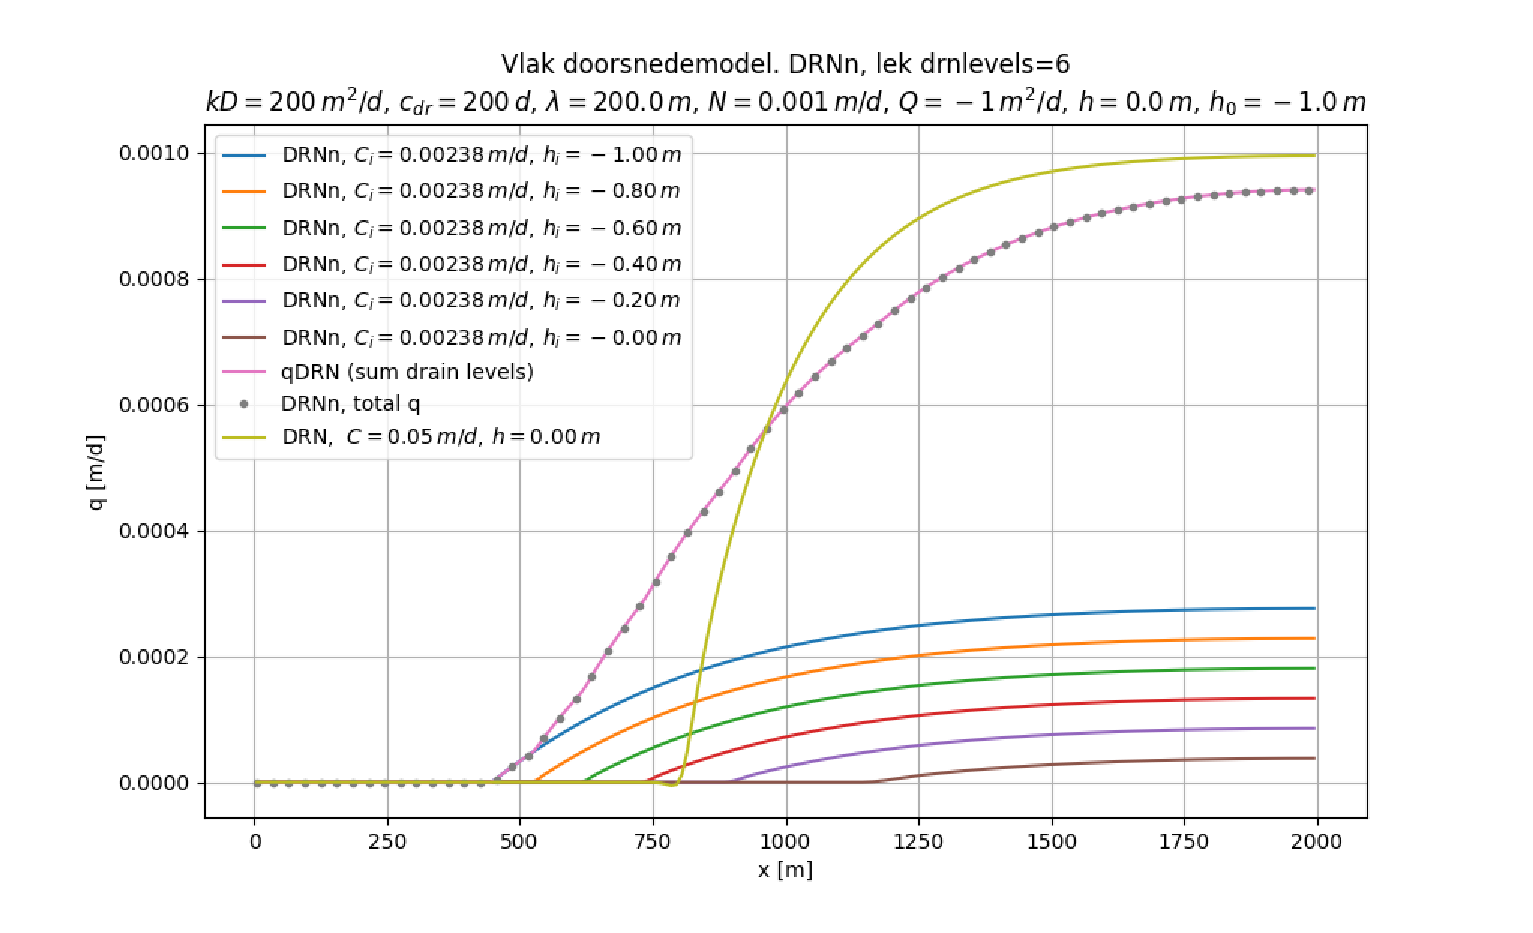
\includegraphics[width=0.8\textwidth]{/Users/Theo/Entiteiten/Hygea/2022-AGT/jupyter/images/example_fdm3_1D_DRNn_leakage}

\caption{\label{fig:Lek-DRNn}Lek in het vlakke doorsnede model voor de situatie
met een drainniveau (groene lijn) en met 6 drainniveau's (paarse lijn
met stippen). De gekleurde lijnen geven de lek afkomstig van de drains
met verschillende drainniveau's. De drains op de verschillende drainniveau's
hebben dezelfde conductantie, zodanig dat de lek bij de referentiegrondwaterstand
($\phi_{N}=h+Nc=0.2$ m) in beide modellen gelijk is.}

\end{figure}


\subsection{De axiaal-symmetrische doorsnede}

De axiaal-symmetrische doorsnede werkt qua invoer hetzelfde als de
vlakke doorsnede, met uitzondering van de analytische oplossing die
voor de situatie met GHB overeenkomt met de Glee plus $Nc$

\[
\phi=h+Nc-\frac{Q}{2\pi kD}K_{0}\left(\frac{r}{\lambda}\right),\,\,\,\lambda=\sqrt{kDc_{dr}}
\]

Figuur \ref{fig:Ax-symm-dsn} geeft het resultaat. De analytische
oplossing valt samen met de numeriek met GHB randvoorwaarden en de
analytische oplossing volgens Blom valt samen met de numerieke met
DRN randvoorwaarden. De straal waarbinnen de grondwaterstand onder
de drains is getrokken is aangegeven met de verticale lijn. Dit punt
komt overeen met een verlaging gelijk aan $Nc$. De onderste figuur
geelt de lek. Voor het model met de DRN randvoorwaarde is de lek gelijk
nu binnen de zojuist genoemde radius. Voor het model met de GHB randvoorwaarde
is wel infiltratie mogelijk waar de grondwaterstand zakt onder het
slootpeil. Voor de analytische oplossing volgens Blom is de voeding
van de watervoerende laag weergegeven. Deze is nul waar de sloten
het volledige neerslagoverschot afvoeren en is gelijk aan het neerslagoverschot
waar de sloten niets afvoeren. De som van voeding en lek is voor Blom/DRN
gelijk aan het neerslagoverschot.

\begin{figure}[h]
\centering
\includegraphics[width=0.8\textwidth]{/Users/Theo/Entiteiten/Hygea/2022-AGT/jupyter/images/example_fdm3_axym}

\caption{\label{fig:Axsym-dsn}Analytische oplossingen en Fdm3-simulatie van
axiaal-symmetrische verticale doorsnede. Het Fdm3-model bestaat uit
een enkele modellaag. Voor de gebruikte gegevens zie de kop van bovenste
figuur. Vergelijking situatie met GHB- en DRN-cellen. Boven de stijghoogten
en onder de lek, respectievelijk de voeding.}

\end{figure}

Figuur \ref{fig:Axsym-dsn} geeft dezelfde resultaten weer als figuur
\ref{fig:Ax-symm-dsn} maar nu met die van vrije drainage eraan toegevoegd,
opnieuw voor de twee varianten. Bij variant ,,FDR'' is de drainageweerstand
als wiskundige functie opgelegd: $c_{dr}=\frac{\gamma}{\sqrt{q}}$
en bij variant ,,FDR1'' is de drainageweerstand berekend op basis
van het slootprofiel en de actuele slootdiepte. De verlaging bij vrije
drainage lijkt hier nauwelijks groter dan bij reguliere drainage,
maar dat komt door de veel kleinere verticale schaal van de grafiek
ten opzichte van die bij figuur \ref{fig:Vlakke-dsn+GHB+DRN} voor
de vlakke 1D doorsnede. Deze schaalverschillen zijn het gevolg van
de veel grotere afmaling in het axiaal symmetrische model ten opzichte
van die van het vlakke model. Ook hier zien we dat de lek aan de rechter
zijde gelijk wordt aan het neerslagoverschot.

Figuur \ref{fig:Vlakke-dsn+GHB+DRN} is hetzelfde als figuur \ref{fig:Ax-symm-dsn}
maar met de resultaten van beide varianten van de vrije afwatering
er aan toegevoegd. FDR de variant met wiskundig opgelegde drainageweerstand
($c_{dr}=\frac{\gamma}{\sqrt{q}}$) en FDR1 die waarbij de drainageweerstand
is berekend op basis van het fysieke slootprofiel. Het verschil tussen
beide blijkt heel gering. De grafiek laat zien dat de verlaging bij
vrije drainage, dus wanneer het slootpeil meezakt met de grondwaterstand
of met afnemende lek, is groter dan bij vast slootpeil. De reikwijdte
blijkt belangrijk groter dan bij vast slootpeil. De onderste figuur
laat zien de lek doorgaat tot de verlaging onder de hoogte van de
slootbodem zakt. Het is net of de sloten veel langer nat blijven dan
bij de DRN randvoorwaarde. Maar dat is maar schijn. Het model met
de DRN randvoorwaarde is eenvoudig een slechte representatie voor
vrije afwatering, en datzelfde geldt voor het schema van Blom, eenvoudig
omdat in deze twee benaderingen het slootpeil niet meedaalt met de
grondwaterverlaging en omdat de lek in werkelijkheid niet zomaar stopt
wanneer de grondwaterstand zakt onder het slootpeil in de referentiesituatie.
Kortom modellering van vrije afwatering of lek met de standaard DRN
optie met vast slootpeil of het schema volgens Blom zijn niet geschikt
voor modellering van grondwater dat vrij lekt naar sloten zonder externe
aanvoer, die meeademen met de grondwaterstand en in droge tijden of
bij onttrekking eenvoudig geheel droog vallen.

\begin{figure}[h]
\centering
\includegraphics[width=0.8\textwidth]{/Users/Theo/Entiteiten/Hygea/2022-AGT/jupyter/images/example_fdm3_axym+FDR}

\caption{\label{fig:Axym-dsn+FDR}Resultaten axiaal-symmetrische doorsneden
als in figuur \ref{fig:Ax-symm-dsn} maar met daaraan toegevoegd de
resultaten van de twee varianten met vrije drainage. FDR is de variant
met wiskundig opgelegde drainageweerstand, FDR1 die met de drainageweerstand
berekend op basis van het slootprofiel.}

\end{figure}

Tenslotte bekijken we de gemodelleerde vrije afwatering werkt out
wanneer we deze simuleren met een aantal (in dit geval 6) drainniveau's
binnen en enkele rekencel, zodanig dat de conductantie (reciproke
weerstand) toeneemt met de grondwaterstand boven de slootbodem. Het
resultaat is te zien in figuur \ref{fig:Axym-DRNn}. Het berekeningsresultaat
van de ,,Modflow-methode'', met meer drainniveau's per rekencel
blijkt min of meer perfect overeen te komen met de andere twee varianten
voor het modelleren van vrije afwatering. Dit impliceert dat de methode
gewoon werkt in Modflow.

\begin{figure}[h]
\centering
\includegraphics[width=0.8\textwidth]{/Users/Theo/Entiteiten/Hygea/2022-AGT/jupyter/images/example_fdm3_axym+FDR+DRN1}

\caption{\label{fig:Axym-DRNn}Grondwaterstand en lek in de axiaal-symmetrische
doorsnede berekend met dezelfde randvoorwaarden als figuur \ref{fig:Vlakke-dsn+GHB+DRN}
maar met daaraan toegevoegd de berekening met vrije afwatering overeenkomstig
Modflow, waarbij de conductantie in 6 stapjes vanaf de slootbodem
toeneemt met de grondwaterstand zodanig dat de afvoer bij de referentiestijghoogte
gelijk is aan het neerslagoverschot, evenals dat voor de andere berekeningsvarianten
het geval is.}

\end{figure}

Figuur \ref{fig:Axym-voeding} geeft de voeding van het watervoerende
pakket voor het model met alle toegepaste randvoorwaarden. Het is
een resultaat van dezelfde simulaties als in de voorgaande figuur.
De blauwe lijn geeft aan dat bij GHB-randvoorwaarden de voeding evenredig
is met de verlaging en dus hoog kan oplopen. Daarom is de voeding
verder van de put, bij grotere $r$ bij vrije drainage minder dan
bij de andere randvoorwaarden. Waar de grondwaterstand bij de DRN
randvoorwaarde onder het niveau van de drains valt ($\phi<h=0)$ is
de voeding gelijk aan het neerslagoverschot $N=0.001$ m/d. Buiten
deze zone, dus met een verlaging minder dan $Nc$ neemt de voeding
af tot 0 op voldoende grote afstand van de put. De voeding voor vrije
drainage neemt eerder af dan die voor vaste drainage, namelijk vanaf
de afstand waarop grondwaterstand boven de bodemhoogte $h_{0}=0$
van de sloten uitkomt. Het verschil tussen de twee varianten met vrije
drainage en de variant waarbij de conductantie toeneemt met de grondwaterstand
door middel van een aantal drainiveau's per rekencel is bijzonder
gering. De drie varianten voor de simulatie van de vrije drainage
zijn in de praktijk equivalent. Vrije drainage kan gemakkelijk met
Modflow worden gesimuleerd door gebruik te maken van meerdere drainageniveau's
per rekencel, dus door meer DRN randvoorwaarden aan dezelfde rekencel
toe te kennen. Als laatste conclusie: het verschil tussen vaste en
vrije drainage is echter aanzienlijk, en dat is het gevolg van het
meedalen van het slootpeil met de grondwaterstand en de daarbij horende
afname van de conductantie, respectievelijk de toename van de intreeweerstand
tussen watervoerend pakket en de sloten.

\begin{figure}[h]
\centering
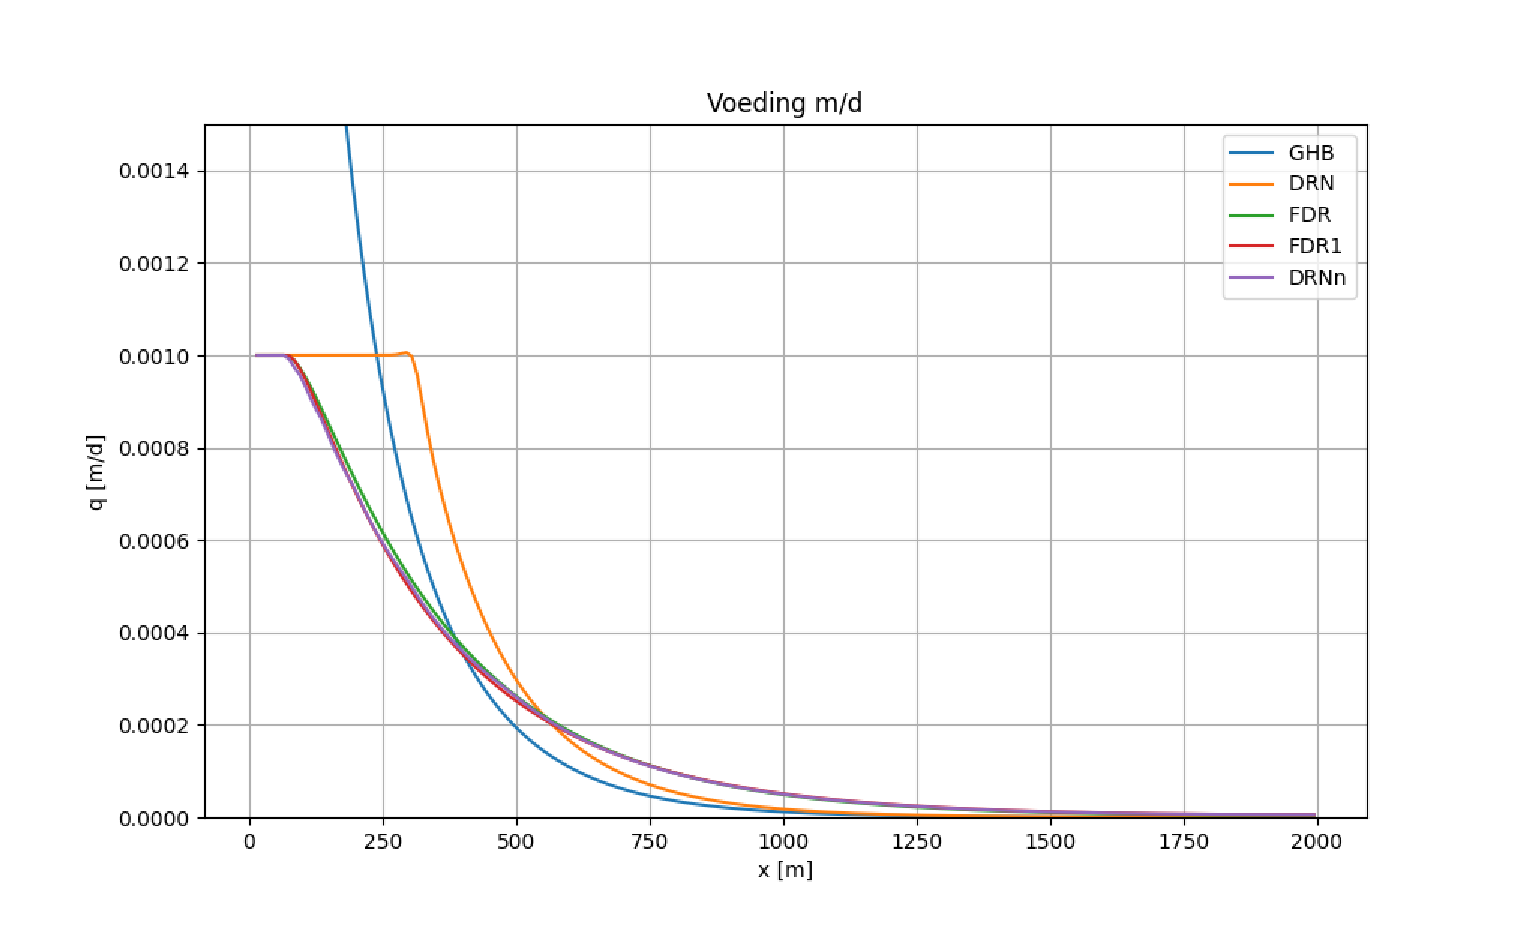
\includegraphics[width=0.8\textwidth]{/Users/Theo/Entiteiten/Hygea/2022-AGT/jupyter/images/example_fdm3_axym_voeding}

\caption{\label{fig:Axym-voeding}Axiaal-symmetrische doorsnede, voeding van
de aquifer voor alle varianten }

\end{figure}

Figuur \ref{fig:Axsym_lek_DRNn} geeft de lek voor de situatie met
een enkele DRN per rekencel en met 6 drainniveau per rekencel zodanig
dat de lek bij de referentiestijghoogte $\phi_{N}$ gelijk is aan
het neerslagoverschot. De groene lijn is die voor de berekening met
een enkel drainniveau en de paarse lijn met puntjes die voor de situatie
met 6 drainniveau's. De totale lek is in beide gevallen gelijk aan
het totale neerslagoverschot op het model minus de onttrekking. Dit
is hier niet direct te zien omdat voor een gemakkelijker inzicht de
lek steeds is gedeeld door $2\pi r$ zodat het antwoord in m/d wordt
verkregen. De gekleurde lijnen geven de lek voor elk van de 6 drainniveau's
(zie legenda). De som van de gekleurde grafieken is gelijk aan de
paarse met de balletjes. De bruine lijn is het hoogste drainniveau.
Het is duidelijk dat dit het eerste droogvalt, voor $r<500$ m. De
blauwe lijn is de lek via de drains met het laagste drainniveau. Deze
lekken het meest omdat het verschil tussen de grondwaterstand en dit
laagste drainniveau het grootst is, terwijl alle drains dezelfde conductantie
hebben (zie legend). Het drainniveau van de blauwe lijn ($h_{i}=-1$
m) valt pas droog voor ca. $r<60$ m.

,
\begin{figure}[H]
\centering
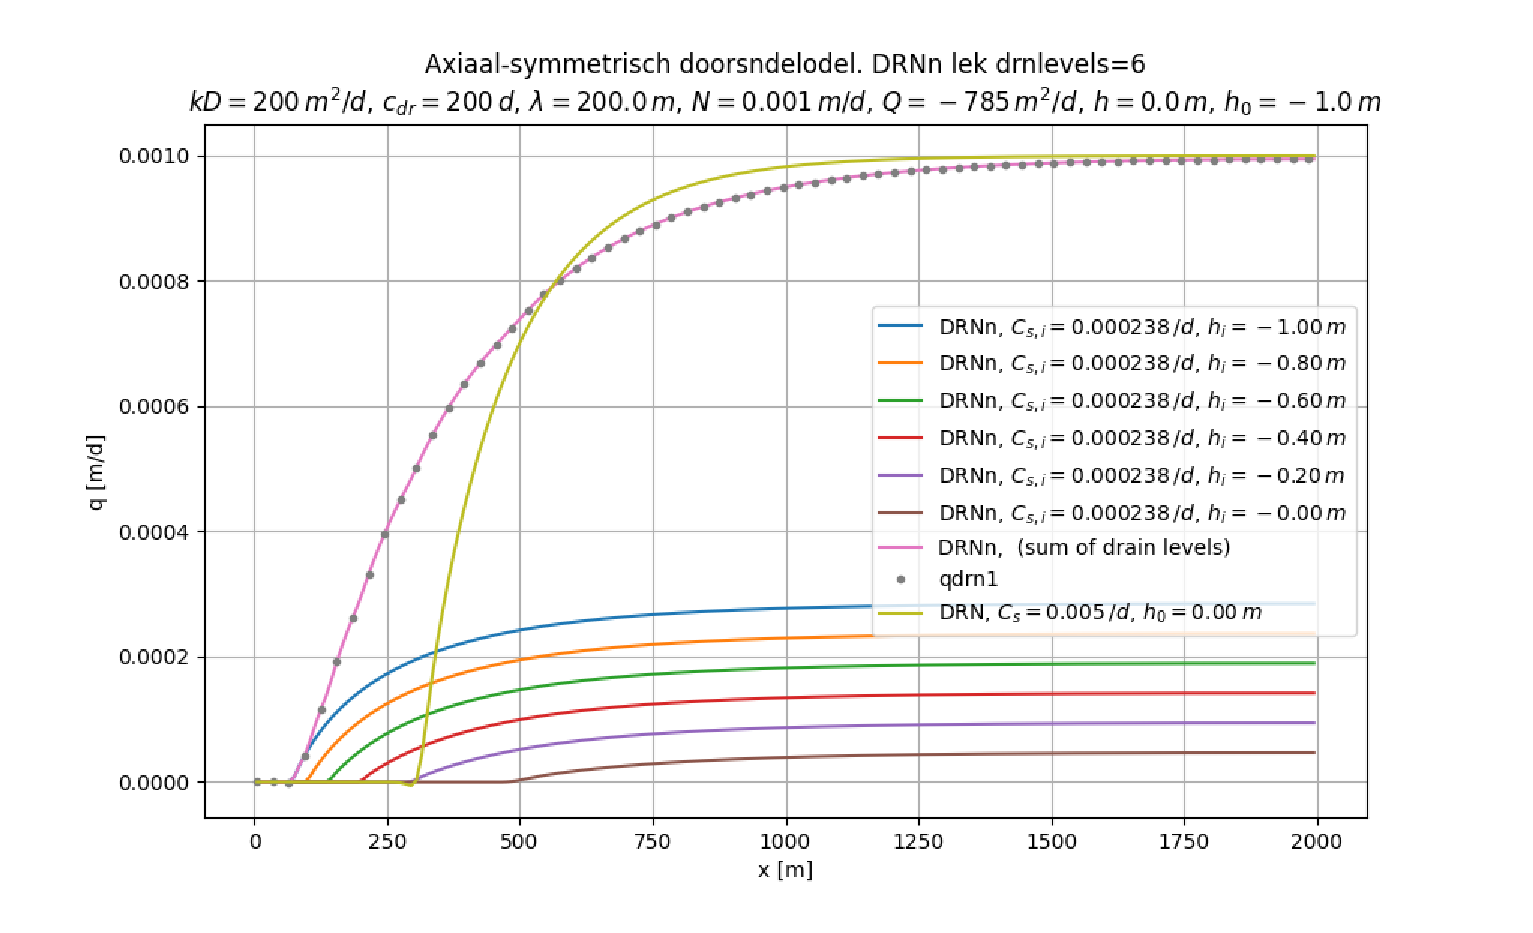
\includegraphics[width=0.8\textwidth]{/Users/Theo/Entiteiten/Hygea/2022-AGT/jupyter/images/example_fdm3_axym_DRNn_leakage}

\caption{\label{fig:Axsym_lek_DRNn}In detail de voeding (aanvulling) van het
watervoerende pakket in de axiaal-symmetrische situatie voor de verschillende
typen randvoorwaarden.}
\end{figure}


\section{Inclusief de Modflow manier met meerdere drainniveau's binnen een
rekencel}

Figuur \ref{fig:vlak-1D-drn1} is dezelfde als figuur \ref{fig:Vlakke-dsn+GHB+DRN},
maar met daaraan toegevoegd het ,,Modflow resultaat'' (lijn Numeriek
DRN1), waarin de vrije afwatering is gesimuleerd met 6 drainniveau's
binnen elke cel zoals weergegeven in figuur \ref{fig:vlak-1D-drn1}
en figuur \ref{fig:Afvoer-vs-phi}. Het blijkt dat noch de verlaging
noch de lek met verschillende drainniveau's met de juiste conductantie
zoals hierboven berekend, nauwelijks afwijkt van de twee andere varianten
met vrije ontwatering. Dit betekent dat de methode om vrije afwatering
in Modflow te simuleren door middel van meerdere drainniveau's binnen
rekencellen volledig werkt.

\begin{figure}[h]
\centering
\includegraphics[width=0.8\textwidth]{/Users/Theo/Entiteiten/Hygea/2022-AGT/jupyter/images/example_fdm3_1D+FDR+DRN1}

\caption{\label{fig:vlak-1D-drn1}Grondwaterstand (boven) en afvoer (onder)
in een vlakke 1D doorsnede. De lijn ,,Lek Numeriek DRN1'' is berekend
met 6 drainniveau's. De resultaten voor deze ,,Modflow variant''
wijken nauwelijks af van de twee eerder ontwikkelde varianten voor
de simulatie van vrije afwatering. De lek valt geheel weg bij een
grondwaterstand $\phi=h_{0}=-1$ m en is gelijk aan het neerslagoverschot
bij een grondwaterstand $\phi_{N}=h+Nc_{dr}=0.2$ m}
\end{figure}

\addcontentsline{toc}{section}{Referenties}
\begin{thebibliography}{Langevin at al. (2017)}
\bibitem[Blom (1973)]{Blom73}Blom, J. (1973). Verlagingen van het
freatisch vlak bij grondwateronttrekking in een gebied met vrije afwatering.
RID mededeling 74-7. Rijkswaterstaat Instituut Drinkwatervoorziening,
Den Haag.

\bibitem[De Glee (1930)]{Glee30}De Glee, C. (1930). De invloed van
grondwateronttrekkingen op de grondwaterstand. Proefschrift, Universiteit
van Amsterdam.

\bibitem[Huisman (1972)]{Huis72}Huisman L. (1972) Groundwater Recovery.
MacMillan. New York etc., 336p. SBN 333-098870-6. 

\bibitem[Louwyck et al. (2022)]{Lou22}Louwyck A, Vadenbohede A, Libbrecht
D, Van Camp M, Walraevens, K. (2022) The radius of Influence Myth.
Water (2022), 14, 149, httpd://doi.org/10.3390/w14020149. httops://www.mdpi.com/journal/water.
27p.

\bibitem[Langevin at al. (2017)]{MF6}Langevin et al. (2017) Documentation
for the Modflow 6 Groundwater Flow Model. Chapter 55 of Section A,
Groundwater, Book 6, Modeling Techniques. Techniques and methods 6-A55.
U.S. Geological Survey. Reston, Virginia, 2017.

\end{thebibliography}


\end{document}
